% REMEMBER: You must not plagiarise anything in your report. Be extremely careful.

\documentclass{l4proj}

    
%
% put any additional packages here
%

\begin{document}

%==============================================================================
%% METADATA
\title{A Sailing Race Manager}
\author{Hamish Philip}
\date{March 24, 2023}

\maketitle

%==============================================================================
%% ABSTRACT
\begin{abstract}
    Castle Semple Sailing Club on Lochwinnoch, Scotland, currently uses a desktop application called Sailwave to score their races. This program has many issues, and the club desires a better system. The goal of this project is to design and build an improved system, that the sailing club can use.

    A system to meet the requirements of Castle Semple Sailing Club was designed and developed. The resulting product was deemed to successfully meet the client's requirements of a system that can replace the system they currently use. Several issues were identified with the final product that decrease its usability. Despite this, the overall system functions to the satisfaction of the customer, and it has solved the problem which this project set out to solve.
\end{abstract}

%==============================================================================

% EDUCATION REUSE CONSENT FORM
% If you consent to your project being shown to future students for educational purposes
% then insert your name and the date below to  sign the education use form that appears in the front of the document. 
% You must explicitly give consent if you wish to do so.
% If you sign, your project may be included in the Hall of Fame if it scores particularly highly.
%
% Please note that you are under no obligation to sign 
% this declaration, but doing so would help future students.
%
\def\consentname {Hamish Philip} % your full name
\def\consentdate {March 24, 2023} % the date you agree
%
\educationalconsent


%==============================================================================
\tableofcontents

%==============================================================================
%% Notes on formatting
%==============================================================================
% The first page, abstract and table of contents are numbered using Roman numerals and are not
% included in the page count. 
%
% From now on pages are numbered
% using Arabic numerals. Therefore, immediately after the first call to \chapter we need the call
% \pagenumbering{arabic} and this should be called once only in the document. 
%
% Do not alter the bibliography style.
%
% The first Chapter should then be on page 1. You are allowed 40 pages for a 40 credit project and 30 pages for a 
% 20 credit report. This includes everything numbered in Arabic numerals (excluding front matter) up
% to but excluding the appendices and bibliography.
%
% You must not alter text size (it is currently 10pt) or alter margins or spacing.
%
%
%==================================================================================================================================
%
% IMPORTANT
% The chapter headings here are **suggestions**. You don't have to follow this model if
% it doesn't fit your project. Every project should have an introduction and conclusion,
% however. 
%
%==================================================================================================================================
\chapter{Introduction}

% reset page numbering. Don't remove this!
\pagenumbering{arabic} 

In the UK, sailing races are scored with rules set by the Royal Yachting Association (RYA).
This scoring method results in many calculations which can be tedious to do by hand. As a result of this, most scoring is done using computer systems \citep{RYAscore}.

\begin{figure}[H]
    \centering
    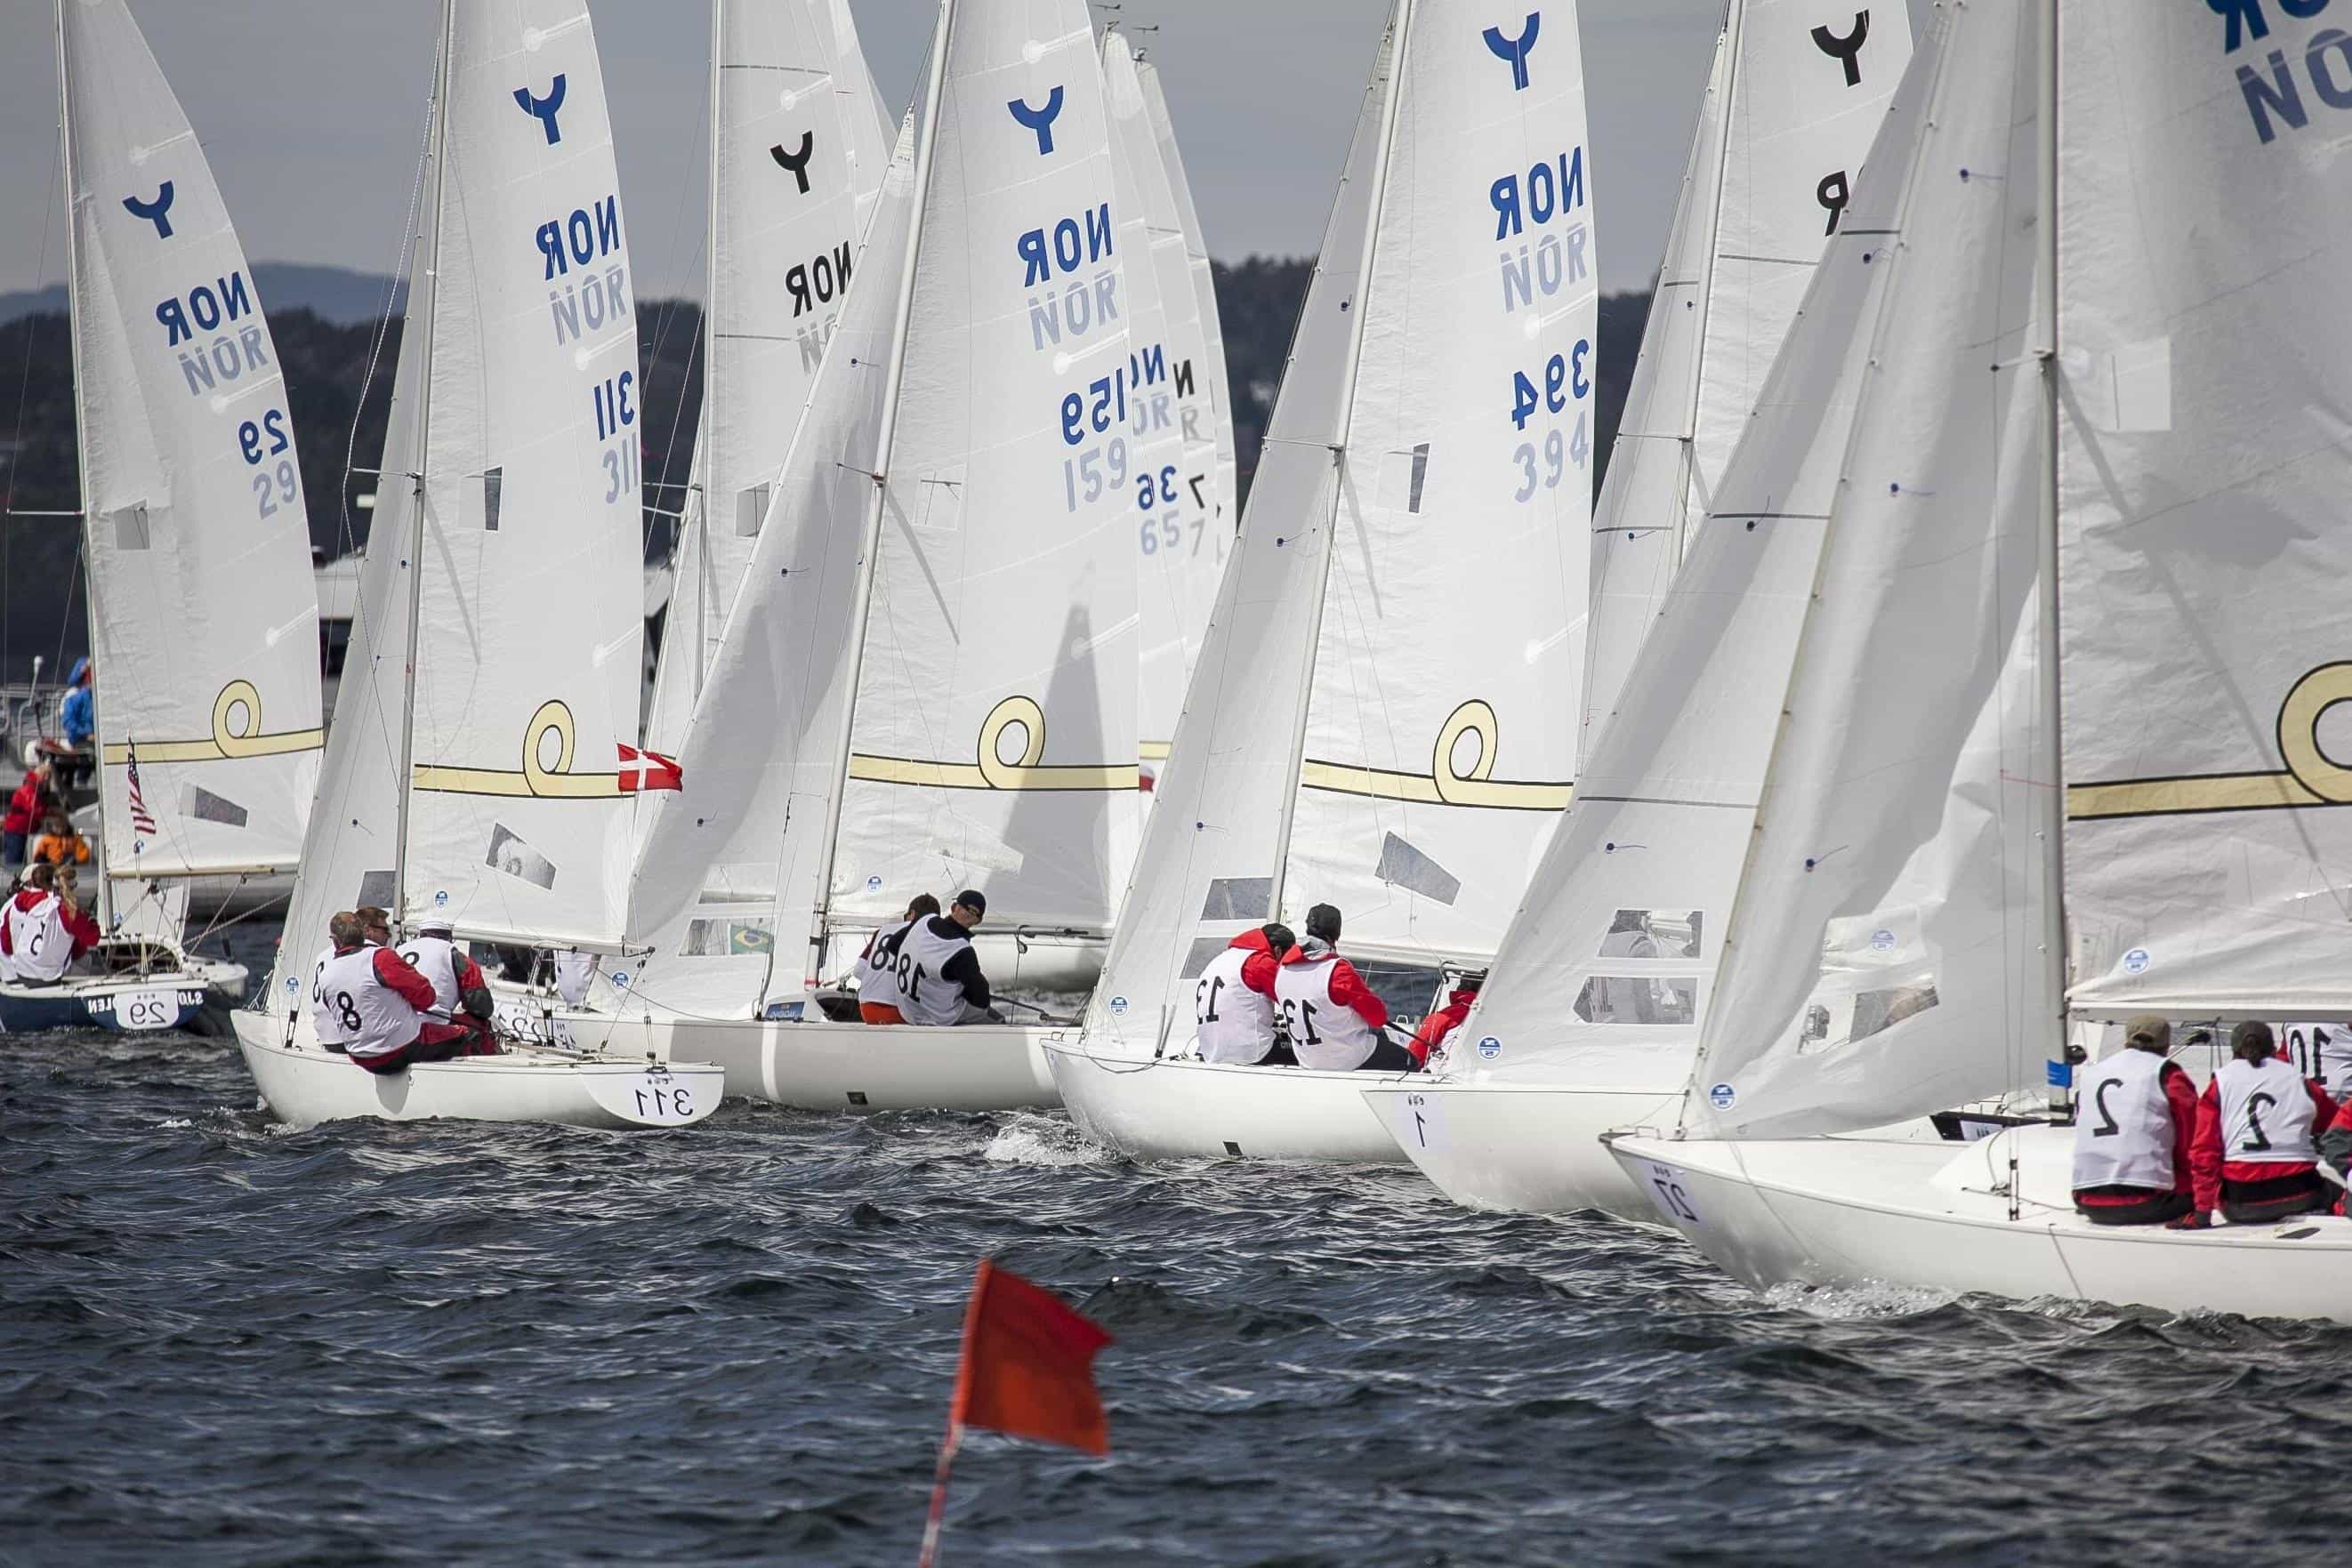
\includegraphics[width=0.7\linewidth]{images/SailingRace.jpg} 

    \caption{A Dingy Sailing Race \citep{SailingRace}
    }

    % use the notation fig:name to cross reference a figure
    \label{fig:SailingRace} 
\end{figure}

Castle Semple Sailing Club on Lochwinnoch, Scotland, currently uses a desktop application called Sailwave to score their races. This program has many issues, and the club desires a better system. The goal of this project is to design and build an improved system, that the sailing club can use.

\section{The Client}
The Client for this project is Castle Semple Sailing Club. Located on Lochwinnoch near Glasgow, Scotland, It hosts many races and events throughout the year and uses a variety of different classes of dinghy. The majority of Castle Semple Sailing Club members have limited computer skills, which needs to be taken into account when designing the solution.

The main point of contact with the club is Dr Simon Rogers, a member of the Castle Semple Sailing Club Committee. He was previously a senior lecturer at the School of Computing Science at the University of Glasgow, and so he has technical knowledge that is relevant to the project. However, he is not able to spare the time to be directly involved in the project, so interaction with him is limited. 

\section{The Problem}
The RYA recommends a certain set of rules to be used when conducting and scoring races, set out in a publication entitled "RYA racing rules guidance" \citep{RYAscore}. The following is a summary of these rules:

A sailor receives points based on their finishing position (1 points for 1st, 2 points for 2nd etc.). The sailor with the lowest number of points at the end of a series (a collection of races) wins that series. Their place in the race is determined by the time they took to complete it, which is corrected by a handicap, so sailors in different boats with different capabilities can race fairly. These handicaps are set by the RYA, and in the case of dingy sailing, are known as the Portsmouth Yardstick Scheme \citep{RYApy}.

Additionally, a sailor can choose to not participate in any number of races in a series, in which case they are awarded a number of points that is greater than the points which any sailor who did compete received. A sailor can also start, but not finish, a race, in which case they are awarded a slightly smaller number of points than not participating. Finally, a sailor can also be involved in running the race, in which case they are given a medium amount of points to reflect their contribution.

The current software, Sailwave, that the sailing club uses has a few limitations. Firstly, as it is a desktop program, it is limited to use on a computer that is owned by the club. This computer is old and slow, resulting in poor performance of the program, and cannot be easily replaced.

\begin{figure}[H]
    \centering
    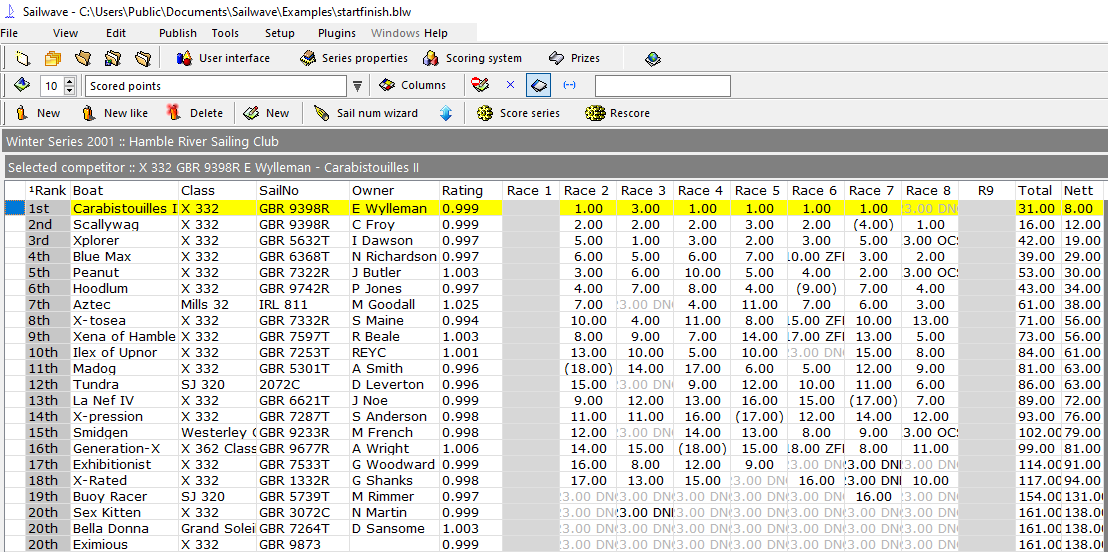
\includegraphics[width=1\linewidth]{images/Sailwave.png} 

    \caption{Main screen of the Sailwave Program \citep{sailwave}
    }

    % use the notation fig:name to cross reference a figure
    \label{fig:Sailwave} 
\end{figure}

Additionally, the software itself is outdated and clunky, having been originally made in 2001 \citep{sailwave}. This can be seen in figure \ref{fig:Sailwave}, which shows the main screen of the Sailwave program. Notice how it is cluttered and confusing. 

In order to distribute the results of a race or series to the participants, the results need to be printed out and manually sent out via another channel, such via email by posting the results on a notice board. This is not ideal, as it adds work for the race administrator, and it reduces the availability of the results. A final problem is that the users of the software at Castle Semple Sailing Club have limited computer skills, so updating the program, moving the program to a new pc or selecting a new program to use is difficult.

This project sets out to design a new sailing race managing system, that solves the problem of calculating a leader board from data collected from races, using the system specified by the RYA. The system must improve upon Sailwave, and should provide some other features that the Castle Semple Sailing Club desires.


%==================================================================================================================================
\chapter{Background}\label{chap:Back}
In this section, we will provide some further background on sailing races, scoring systems and identify some resources that may be useful in development of this project. 

\section{Sail Racing}
The official rules for sailing races, known as The Racing Rules of Sailing, are set out, and updated every 4 years, by World Sailing, the international authority for the sport. Certain deviations from these rules are allowed to be made by Member National Authorities, which for the UK, is the Royal Yachting Association (RYA). The RYA publishes these rules in a document called RYA Racing Rules Guidance \citep{RYAscore}.

In general, a sailing race works by participants sailing round a set course. This can be small as in a dinghy race, or go all the way around the world, such as in the Golden Globe Race. The time participants take to sail around the course is measured. This time is then adjusted with what is known as a handicap, which accounts for the different sailing abilities of different boats. The boat that took the shortest time, corrected by the handicap, wins.

The RYA provides guidance as to how a sailing race should be scored. This Guidance is based on the rules set out by World Sailing. It is up to the committee organising the race as to which scoring system is used. The recommended and default system to use is the “Low Points System”.

The low points system works by granting the participant in 1st place, with the lowest corrected time, 1 point, the one in second place 2 points etc. Participants can also be awarded a variety of different penalty points in various circumstances, for example not competing in a race, or starting but not finishing. The full set of circumstances and the associated points are specified in the RYA racing rules guidance document \citet{RYAscore}.

Multiple races form a series, often known as tournament in other sports. The participants' points from all the races in the series are added together, and the one with the lowest number of points wins. In this way, a participant need not compete in every race in a series in order to take part, but for every race they do not compete in, their score will increase due to the penalty points.

Handicaps, how they work, their history and how they are calculated are explained in the paper “Sailing close to the statistics” \citep{hanicaps}. Wolstenholme says that handicaps allow boats with different capabilities to race against each other fairly, separating the performance of the boat from the performance of the crew. 
According to \citet{hanicaps}, a common handicap method is a time-on-time approach. This is where a time correction is applied to a boat’s finishing time. This is the method recommended by the RYA.

The exact method generally used in dinghy sailing in the UK is the Portsmouth Yardstick Scheme, which was created in 1951 \citep{hanicaps}. In this system, handicaps are given as a number close to 1000. An extract from the Portsmouth Yardstick Scheme Number list \citep{RYApy} can be seen in figure \ref{fig:Hanicaps}

To use the handicaps from provided by the scheme to calculate a corrected time, The following formula is applied to the time in seconds:

\begin{equation}
    \text{Corrected Time(seconds)} = \frac{\text{Time(seconds)} \times 1000}{\text{Handicap}},
    \label{eq:1}
\end{equation}  

This formula means handicap values under 1000 increase the time, thus slowing boats down, and those over 1000 reduce it, thus speeding boats up. The result is the corrected time in seconds, which is used in scoring \citep{RYAscore}.

\begin{figure}[H]
    \centering
    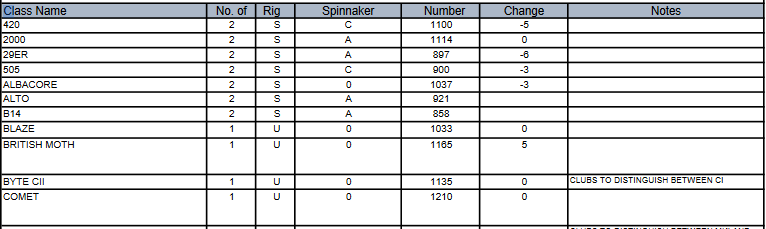
\includegraphics[width=1\linewidth]{images/Handicaps.png} 

    \caption{Extract from the Portsmouth Yardstick Scheme handicap number list \citep{RYApy}
    }

    % use the notation fig:name to cross reference a figure
    \label{fig:Hanicaps} 
\end{figure}

Historically, handicaps have been calculated either using past performance, or on the physical design of the boat. The Portsmouth Yardstick scheme updates their handicaps based on past club race results, and updates them every year \citep{hanicaps}.

\section{Scoring systems}
The underling problem to a sailing race manager is simply a system that records and displays results. Many of these exist across many different sports. By looking at some of these systems, we can get an idea of what makes a scoring system, that can be used to inform this project.

One example is part of the website of the Lawn Tennis Association \citep{Tennis}, which displays the results of tennis torments. A screenshot from the website is pictured in figure \ref{fig:Tennis} below.

\begin{figure}[H]
    \centering
    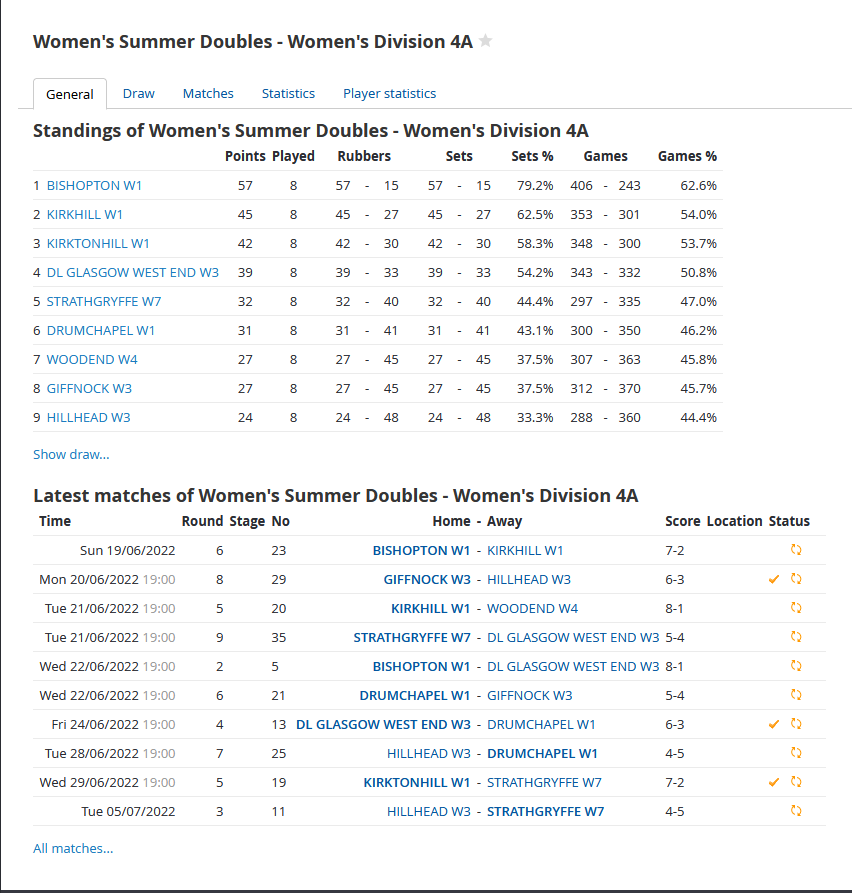
\includegraphics[width=0.6\linewidth]{images/Tennis systme.png} 

    \caption{results page of LTA Women's Summer Doubles \citep{Tennis}
    }

    % use the notation fig:name to cross reference a figure
    \label{fig:Tennis} 
\end{figure}

It can be seen that the page consists of a table, listing the participants in the order of who is winning, along with some score statistics. This is a simple formula that most scoring systems seem to follow.

Another example is the results page on the website of the Victoria Park Run, Glasgow, which is shown below in figure \ref{fig:parkrun}.

\begin{figure}[h!]
    \centering
    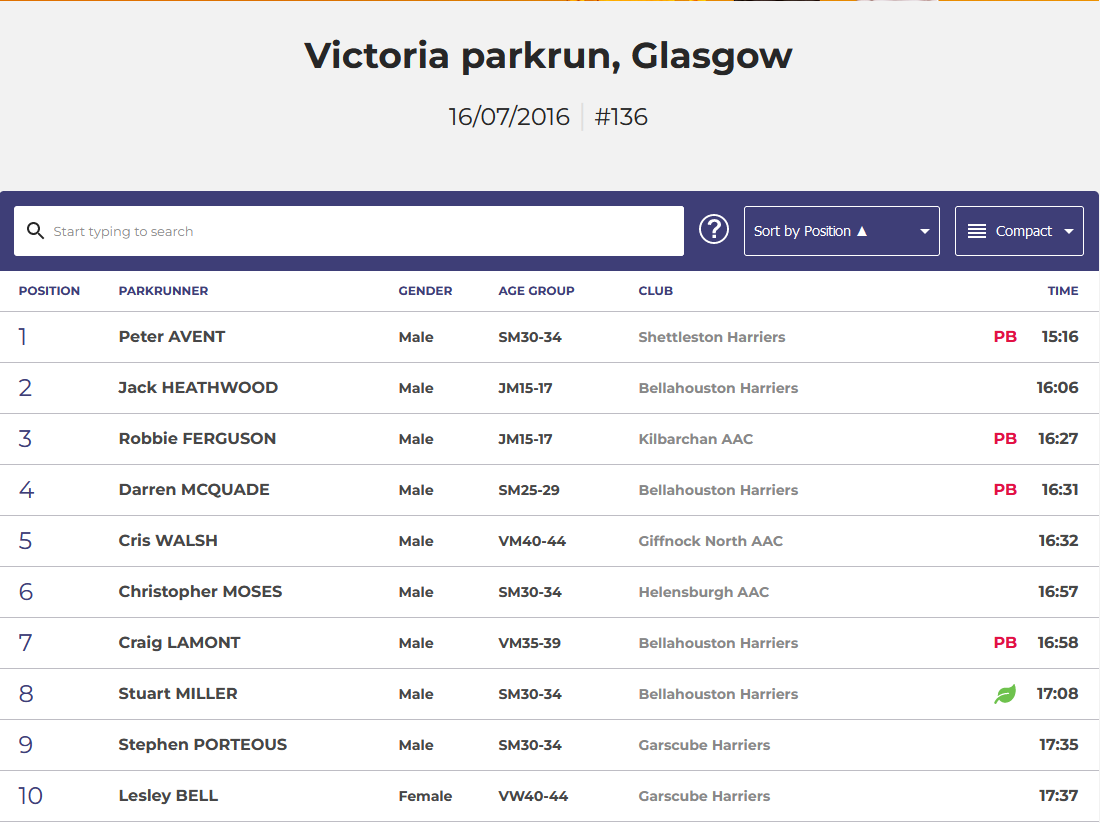
\includegraphics[width=0.6\linewidth]{images/ParkRun.png} 

    \caption{results page of the Victoria Park Run, Glasgow \citep{Parkrun}
    }

    % use the notation fig:name to cross reference a figure
    \label{fig:parkrun} 
\end{figure}

This results page looks much the same as that from the Lawn tennis association \citet{Tennis}. List of participants, ordered by who is winning, with some relevant statistics. The part of this project that involves displaying the results is conceptually similar to these two examples.

The previous two examples are just results pages, whereas this project is also concerned with a system to calculate those results. A closer example to this project can be found in a dissertation by Ying Lu \citet{Multi-sport} which developed a system to manage multi-sport events, such as a triathlon. It resulted in a system that could organize different races, calculate results and display them. This is a similar problem to that this project is trying to solve.

\section{Currently existing Sailing race Management systems}
Diving more deeply into scoring systems in the context of sail racing, a number of systems already exist. These can be drawn on for inspiration. Detailed analysis of three of these systems to inform the requirements for this project made in the next chapter \autoref{chap:A/R}.

\section{Development Resources}

Two likely web-app frameworks to use for the project are Django and Flask. The Django website \citep{django} and the website for flask by \citet{flask} provide a wealth of information about each framework, that can be used to decide which one would be the best to use. The \citet{django} website says that Django is a high-level python framework that encourages rapid and clean web development. The \citet{flask} website says that flask is a lightweight application framework, designed to make getting started quick and easy.

Django was selected as the best one to use. The reasons for this are given in detail in \ref{chap:imp}. The Textbook "Tango with Django" by \citet{tango} provides great instruction in using the Django framework. This book is incredibly useful, as the Django framework is the one this project will be using.

A possible development method is the agile methodology. This methodology is explained well in a paper by \citet{agile}. The paper says that the main things that characterise an agile methodology are:
\begin{itemize}
    \item 
    Individuals and interaction over process and tools.
    \item 
    Working software over comprehensive documentation.
    \item 
    Customer collaboration over contract negotiation.
    \item 
    Responding to change over following a plan.
\end{itemize}

Following this methodology could help ensure an effective development process for the project.

Docker is used for the deployment of the project. Docker is explained well in a paper by \citet{docker}. It essentially allows for simple and quick deployment, as all dependencies are contained within the docker container.




%==================================================================================================================================
\chapter{Analysis/Requirements}\label{chap:A/R}
\section{Analysis of Current solutions}
In this section, we will take a closer look into three currently existing sailing race management systems, and identify what can be learned from how they approached this problem.
\subsection{Sailwave}
Sailwave \citet{sailwave} is the software currently used by Castle Semple Sailing Club. It is free, but closed source, software, originally released in 2001.
The front page of its website \citep{sailwave} states: “Sailwave is a popular, fully-featured, easy-to-use, multilingual, sailing results/scoring application for Windows from XP to Windows 11“

Sailwave has a large list of features. Some notable ones, also taken from the front page of its website \citep{sailwave} are as follows:
\begin{itemize}
    \item
    Flexible scoring: score across all competitors or by fleet, club, nationality, etc.
    \item
    Publish retirement sheets, competitor lists, alternative penalty sheets, etc.
    \item
    Send your news (reports, results, and photos) directly to the Yachts and Yachting magazine website.
    \item
    Publish directly into programs like Microsoft Word and Excel etc,
    \item
    Publish to web documents (HTML) for upload to websites or printing or emailing. Integrated support for FTP/SFTP/SSH/FTPS.
\end{itemize}

It can be seen that the software contains a myriad of different features and use cases. The front page of its website lists 33 different features, some of which were shown above. It can be deduced from this that the program is overcomplicated, cluttered and confusing.
Figure \ref{fig:SailwaveEmpty} shows the page a user is greeted with upon first startup of the program. There are many bottoms and menus presented in the toolbar, but many are greyed ou, and it is not immediately clear where to start.

\begin{figure}[H]
    \centering
    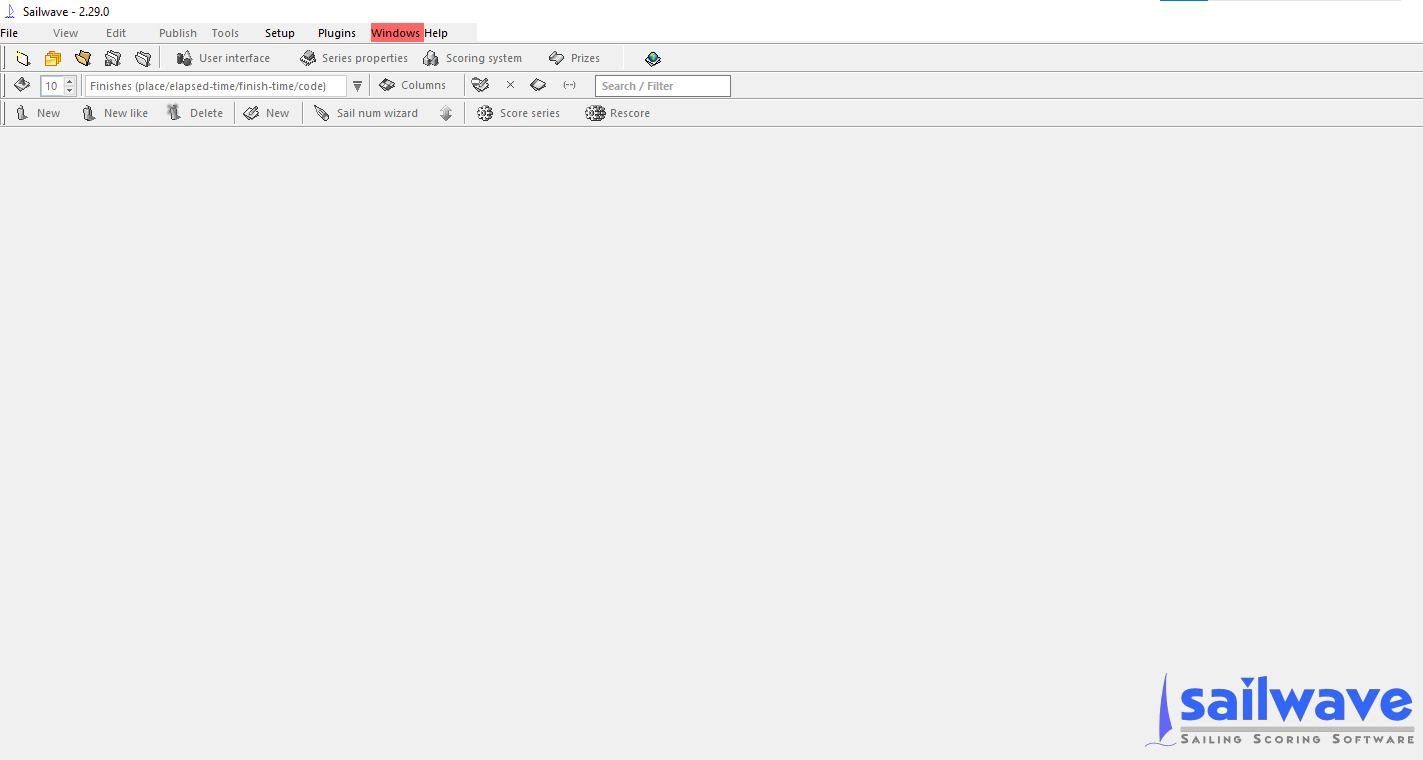
\includegraphics[width=1\linewidth]{images/SailwaveEmpty.png} 

    \caption{Start-up screen of the Sailwave program \citep{sailwave}
    }

    % use the notation fig:name to cross reference a figure
    \label{fig:SailwaveEmpty} 
\end{figure}

Figure \ref{fig:SailwaveEdit} shows Sailwave when a user has started a new series and is attempting to edit one of the entries. A massive amount of different fields are available to be filled out across multiple tabs. It is not clear which cell in the excel-like table corresponds to which entry in the dialogue box. It is clear that Sailwave provides lots of support for various uses, but how much of what Sailwave does, is directly relevant to a small sailing club? The importance of restricting the features of programs is shown in an article by \citet{leanSoftware}. In it, he says that bloated software takes more time to design, code and debug. This can be seen in Sailwave as, to reach its current state, the software has been continually added to over the past 22-years, since its first release in 2001 \citep{sailwave}.

\begin{figure}[H]
    \centering
    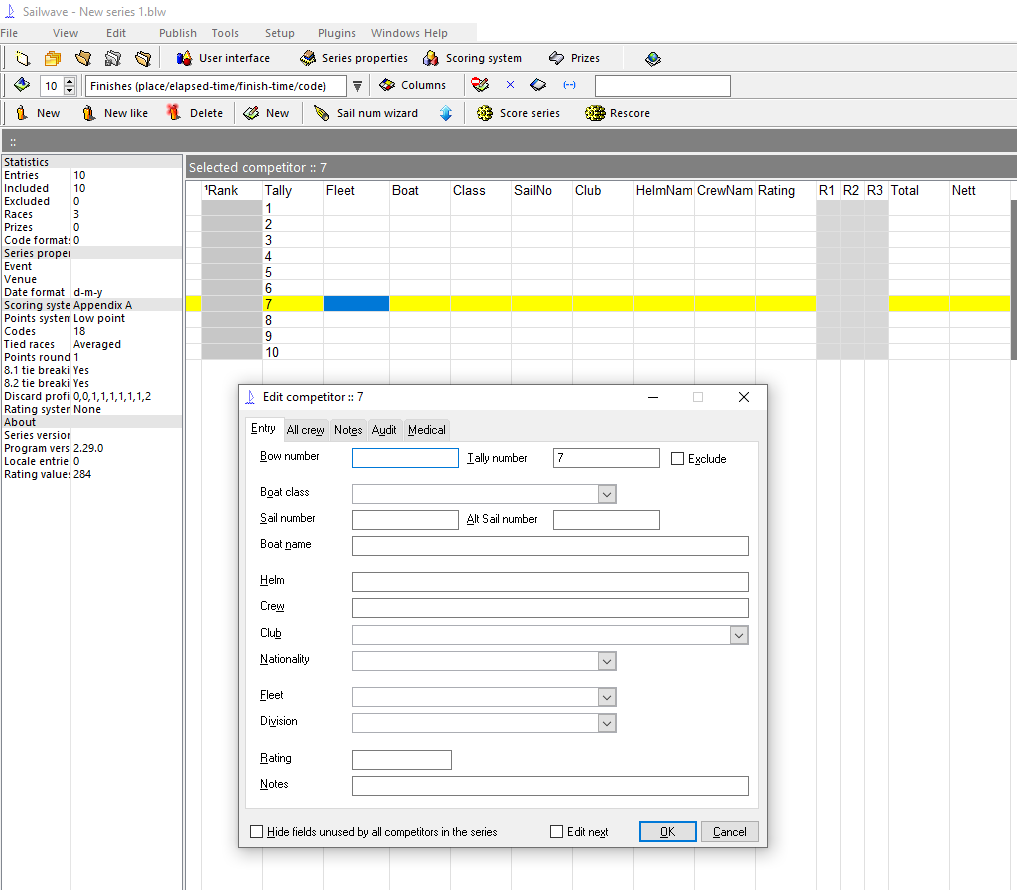
\includegraphics[width=1\linewidth]{images/Sailwave_edit.png} 

    \caption{Editing a cell in the Sailwave Program \citep{sailwave}
    }

    % use the notation fig:name to cross reference a figure
    \label{fig:SailwaveEdit} 
\end{figure}

Sailwave does succeed in presenting some of its information in a clear and easy to understand manner. The main example of this is the race details shown in the excel-like table, as can be seen in figure \ref{fig:Sailwave}. The format of the data resembles a Microsoft Excel spreadsheet \citep{Excel}, an example of which is shown in figure \ref{fig:Excel}. The resemblance is apparent. As many people are familiar with spreadsheets, past skills can make it easier for users to understand Sailwave.

\begin{figure}[H]
    \centering
    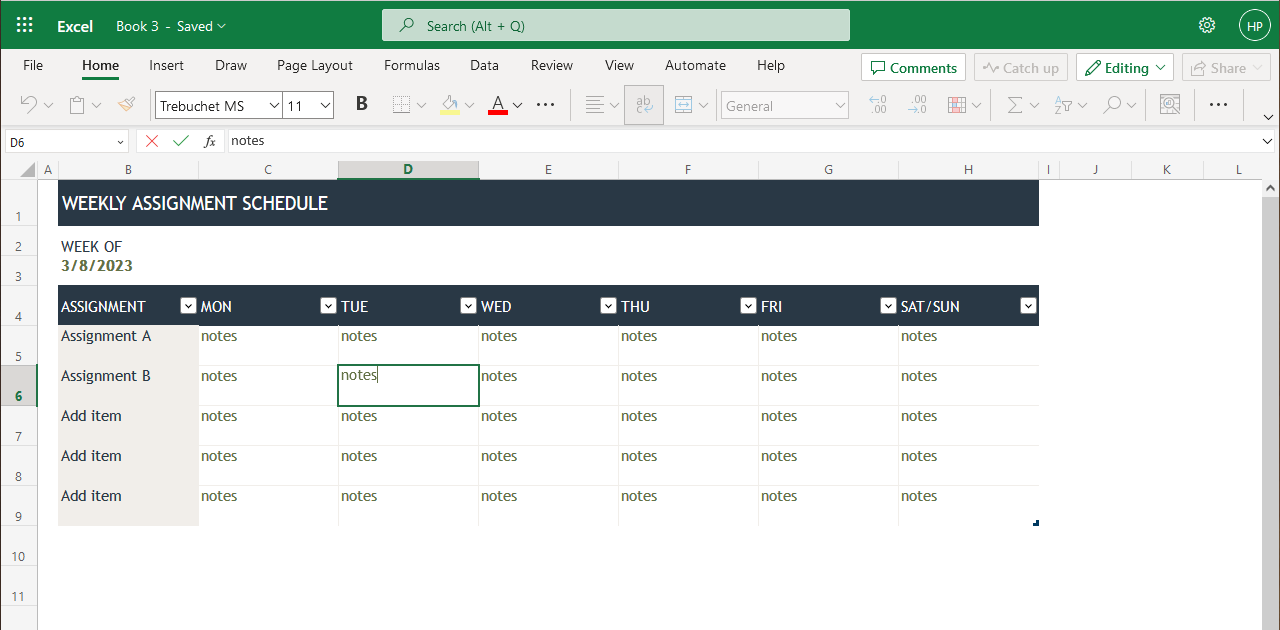
\includegraphics[width=1\linewidth]{images/Ecel.png} 

    \caption{Example of a common Excel spreadsheet \citep{Excel}
    }

    % use the notation fig:name to cross reference a figure
    \label{fig:Excel} 
\end{figure}

Overall, the standardised excel-like format Sailwave uses is a good lesson that can be learned from when designing a new solution, particularly as the members of Castle Semple Sailing Club are already used to Sailwave. We aim to improve on Sailwave by cutting out many of the features that aren't relevant to a small-scale sailing club.

\subsection{Sailing Club Manager}
\citet{ClubManager} is a web-based application that takes a different approach. It seeks to provide a complete platform to manage every part of a sailing club, from race scoring to membership management to morning booking. It is purchased via a subscription.

The scope of Sailing Club Manager is obviously far beyond the problem this project seeks to tackle, as club manager provides features for managing club membership payments, the booking of moorings and the reserving of club boats. It does however show an example of a more professional solution. As Sailing Club Manager is paid software, and doesn't provide any example or demo, it cannot be accessed to analyse and compare it's functionally directly. The explanation of how it works and what it does on its website can still be used as a useful example of a solution with a wider scope.

Focusing in on the race scoring feature, the website \citep{ClubManager}, shown in figure \ref{fig:ClubManager},  lists, among others, the following features:

\begin{itemize}
    \item
    Flexible scoring: score across all competitors or by fleet, club, nationality, etc.
    \item
    It can be used on any device that can browse the internet including tablets, Macs and PCs. 
    \item
    It's easy to use and doesn't require Race officers to learn complicated software. 
\end{itemize}

\begin{figure}[H]
    \centering
    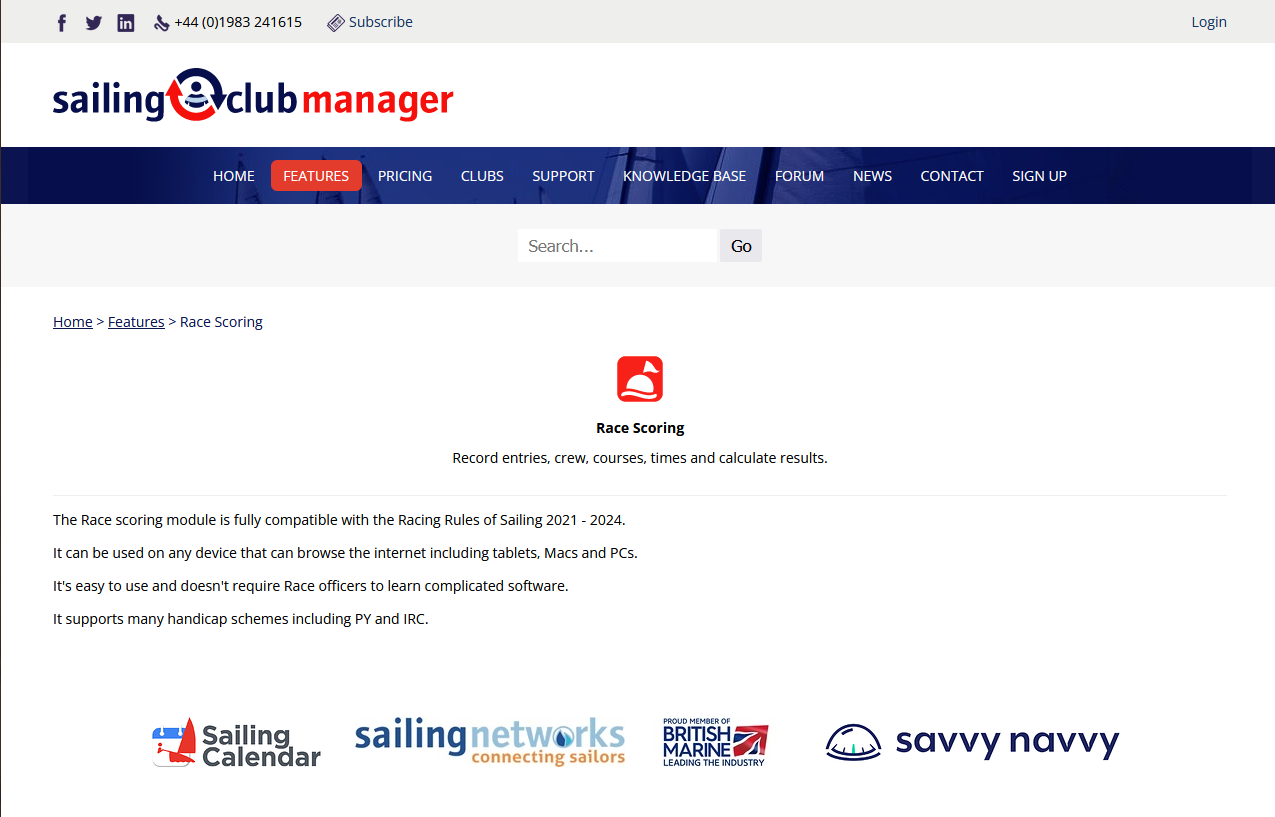
\includegraphics[width=1\linewidth]{images/ClubManager.png} 

    \caption{Race scoring Features page on the Sailing Club Manager Website \citep{ClubManager}
    }

    % use the notation fig:name to cross reference a figure
    \label{fig:ClubManager}
\end{figure}
Compared to Sailwave, the features are much smaller in number, and directed towards a simple use-case. This shows that this software is much more directed towards ease of use and practicality, than Sailwave. Due to the lack of tech skills among the members of Castle Semple Sailing Club, having a new solution take an approach more similar to club manager may be beneficial.

As the scope of Sailing Club Manager far exceeds that of what Castle Semple Sailing Club want, it can be used as an example of what to stay away from. If the scope and features of a new solution begin to resemble that of Sailing Club Manager, then they should be reduced.


\subsection{Sail Event}

Sail Event \citet{SailEvent} is a web-based application that is very similar to Sailwave in what it does. However, it does so in a very different way. It is again a free, but closed source, web-app, with a paid version that provides more features. Users can log in as either a club or a sailor. Clubs can create races, sailors can join them. A screenshot of the user interface where races are created is shown in figure \ref{fig:sailEvent}

\begin{figure}[H]
    \centering
    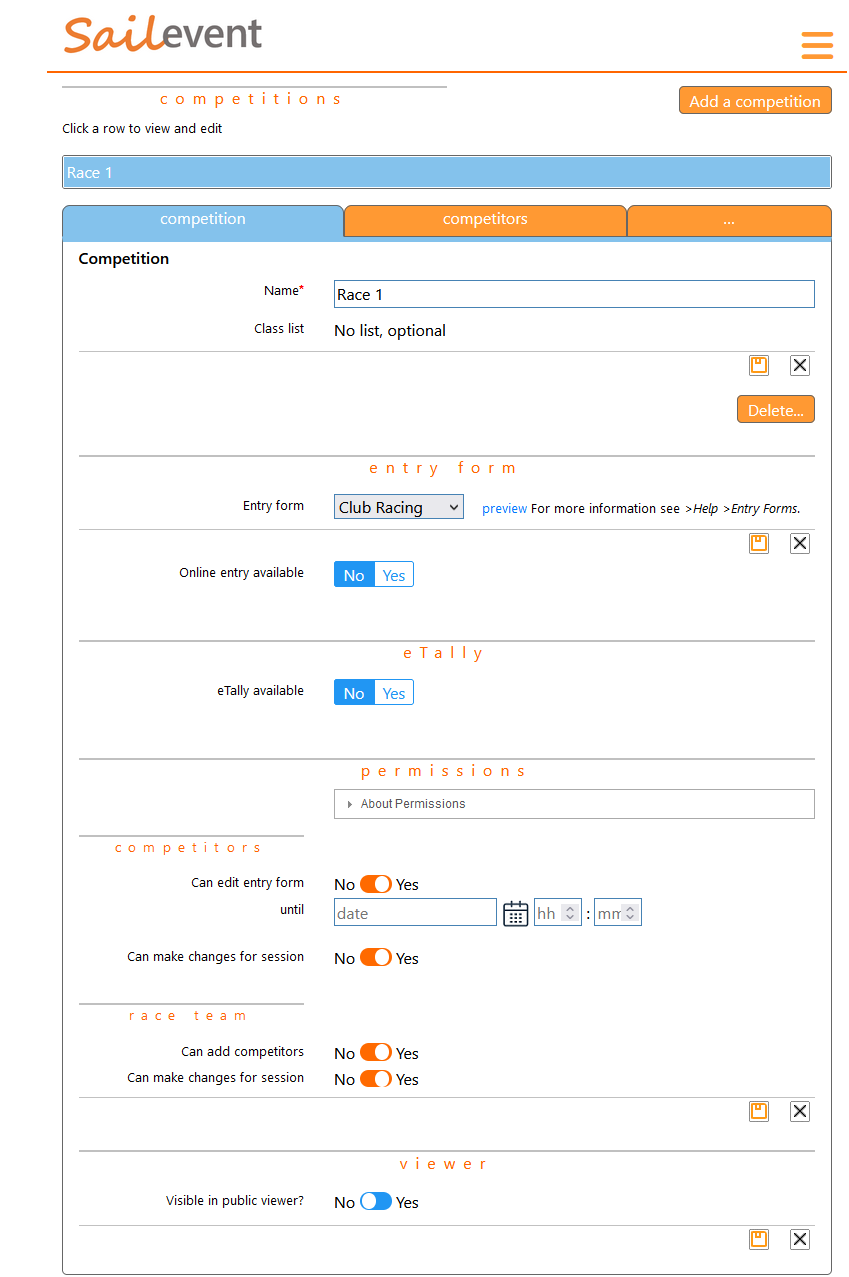
\includegraphics[width=1\linewidth]{images/Sailevent.png} 

    \caption{Race creation page in \citet{SailEvent}
    }

    % use the notation fig:name to cross reference a figure
    \label{fig:sailEvent}
\end{figure}


The figure shows the race creation screen for club users. This differs from its counterpart in \citet{sailwave} as it avoids the spreadsheet-style of data input, and instead uses a list of different fields. This results in a generally less cluttered look, but makes it harder for a user to understand where and what data to input, as they must take in the whole screen, whereas in \citet{sailwave}, a user must only read the column headers to know required.

Due to sail event being a web-app, it has the advantage of being able to be assessed from any device without any set-up, which may well suited to the demographic of Castle Semple Sailing Club, who have limited computer experience to deal with complex software setup.

\subsection{Summary}

Overall, the good features from the three solutions analysed include:
\begin{itemize}
    \item
    spreadsheet-style data entry from \citet{sailwave}.
    \item
    The simple and stream-lined approach from Sailing Club Manager \citet{ClubManager}.
    \item
    The limited features from and uncluttered look of Sail Event \citet{SailEvent}.
\end{itemize}

The things to stay away from in a new system include:
\begin{itemize}
    \item
    Clutter and feature bloat of \citet{sailwave} 
    \item
    The wide scope of Sailing \citet{ClubManager}
    \item
    The hard-to-understand user input \citet{SailEvent}
\end{itemize}

Of all the examined systems, none of them completely meet Castle Semple Sailing Club's needs. By bringing together the good parts of each of these systems, while keeping the overall design close to \citet{sailwave}, a system can be designed that meets all the club's requirements.

\section{Client Meeting}

An initial meeting with the client was held to discuss requirements in October 2022. It was important to make sure the client’s requirements were correctly identified because, as discussed previously, the client will not be available to regularly check on progress, so there is limited ability to revise the requirements before the system is implemented.  At the meeting, the following requirements were identified:

Main requirements
\begin{itemize}
    \item
    Must be a web-app.
    \item
    Race scored with Portsmouth Yardstick handicap and RYA low scoring rules.
    \item
    People can enter races (entered by race admin or do it themselves).
    \item
    People can enter as many or as few races as they like.
    \item
    People can use different boats for each race.
    \item
    The interface for the input of data should look like an interactive excel spreadsheet.
    \item
    Race Participants can access the system to see the leader board.
    \item
    Boats are predefined (drop down menu).
\end{itemize}
Extensions
\begin{itemize}
    \item
    Have the ability for sailors to discard their worst results if there have been enough races.
    \item
    Ability to embed  the leader board in another website.
    \item
    Create an app to help collect times.
\end{itemize}

\section{Initial Plans}
From the initial requirements, two general plans for a system were made.
\subsection{Plan 1}
The first plan was a web-app race manager, very similar to \citet{SailEvent}, with the following features:
\begin{itemize}
    \item
    Admin can create races.
    \item
    Sailors can log in to enter themselves into races and view the leader-board.
    \item
    Separate accounts for Admin + Sailors.
\end{itemize}

This has the advantage of less work for the person managing races than the current system, as sailors enter themselves, and allows the performance of sailors to be tracked across different series.

However, It does stray a little into complete club management, as all the different accounts would have to be managed. For example, who has access to a sailor account, only those who has paid the club fees? This adds complexity.

\subsection{Plan 2}
The second plan was a race management program, similar to what the club is already using in \citet{sailwave}, But hosted in a web-app, with a web-app view of the leader-board. This plan takes inspiration from the Victoria park run website \citeyear{Parkrun} where the results are available publicly, but only someone with an admin account can view them. It would have the following features:
\begin{itemize}
    \item
    desktop-style editor with web-app leader-board, all on the web
    \item
    race manager creates races and enters sailors with admin account
    \item
    without admin account, a sailor can only view the leader-board
\end{itemize}

The advantage of the approach is it greatly decreases complexity as no account managing is needed beyond the admin account. However, the approach does have less functionality than the first plan

\section{The Requirements}
Upon consultation with the client, the second plan was selected as the best approach. The reduction in complexity, from not having to deal with complex account management, was desirable as it means the project is more likely to succeed, with the limited time and
resources available.

Additionally, one of the main problems with the current system, \citep{sailwave}, is that it is complex and packed with far more features than Castle Semple Sailing Club require. In order to design a new system that improves upon this, it in necessary to strictly limit the features to only those which the club requires. This would result in a more lightweight and easy to use system, as required.

To summarise the requirements, a list of user stories is shown below:

Minimum Viable Product
\begin{itemize}
    \item
    Sailor can view the leader-board with a web browser to see who is winning the series.
    \item
    Sailor can view the race results of any race in a series.
    \item
    Race officer can log in to admin account to input information.
    \item
    Race officer can add a new series to start adding races.
    \item
    Race officer can add a sailor to a series so they can enter races.
    \item
    Race officer can add a new race to a series to add race results.
    \item
    Race officer can add a sailor to a race to enter them in the race.
    \item
    Race officer can select which boat the sailor is in to apply
    correct handicap.
    \item
    Race officer can add a sailor’s race time to record a race result.
    \item
    Race officer can remove incorrect sailors, races and series’ to undo mistakes.
    \item
    Race officer can indicate a sailor was a shore officer to give them correct credit.
    \item
    Race officer can indicate a sailor started but didn't finish to give them the correct credit.
    \item
    Race officer can see score of each sailor in the race that is automatically calculated to know the results
    \item
    Race officer can see leader-board automatically updated with scores so that they know the current state of the series
\end{itemize}

Should have

\begin{itemize}
    \item
    A new user can easily install software on their own machine or a cloud platform of their choice to be able to use it.
    \item
    Race officer can define a pattern to exclude worst scoring races if sailor has entered enough of them.
\end{itemize}

Could have
\begin{itemize}
    \item
    A user can embed the leader board of a series in another website to share results easier.
    \item
    Race officer can input race times with an app to make inputting the results in easier.
    \item
    Users can have accounts to track their results across multiple sires.
\end{itemize}

This list encapsulates the requirements of the project that the client desires. For the project to be complete, it should implement all the requirements specified in the "minimum viable product" above. When these are working correctly, the project should then seek to implement the "Should have" and "could have" sections. These represent non-essential requirements, that the system can function without if they cannot be implemented.

%==================================================================================================================================
\chapter{Design}
The first step in the design is to design a database to store all the necessity information about series races, sailors and boats.
\section{Database}

Figure \ref{fig:ERD} shows an entity relationship diagram for the database. 

\begin{figure}[H]
    \centering
    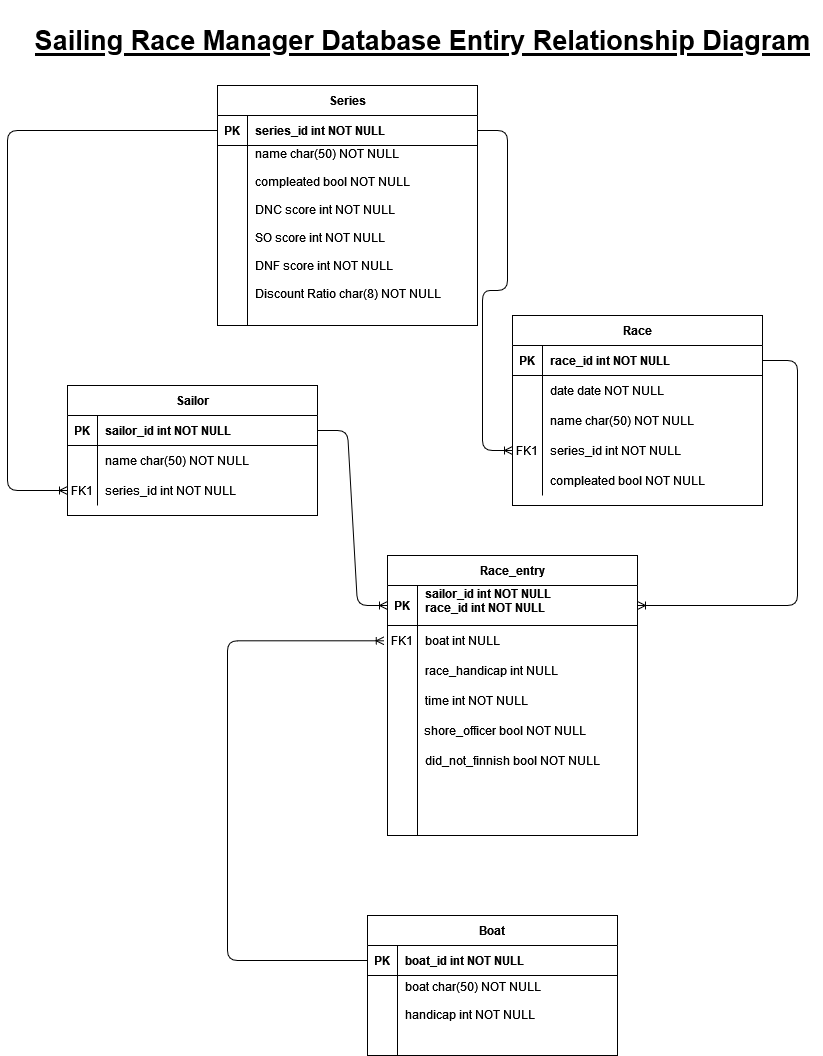
\includegraphics[width=0.75\linewidth]{images/ERD FINAL.png} 

    \caption{Entity Relationship Diagram, showing the different tables in the database, their attributes, and relationships.
    }

    % use the notation fig:name to cross reference a figure
    \label{fig:ERD}
\end{figure}

The following is an explanation of the database:
\begin{outline}
    \1
    Series represents a series of races.
        \2
        The name attribute represents the user-entered name of the series. It is up to the user to know which is which in the case of non-unique names.
        \2
        The ongoing attribute represents if the series is still in progress. This should only affect the displaying of the series data.
        \2
        The DNC score attribute (Did not compete) defines the penalty score for not competing in the series. As this is defined per series, it means that different series can have different values for this and the other penalty score attributes, increasing the flexibility of the software.
        \2
        The SO score attribute (Shore officer) defines the penalty score for being a shore officer in a race.
        \2
        The DNF score attribute (Did not finish) defines the penalty score for starting, but not finishing, a race.
        \2
        The discount ratio attribute defines how many races must be competed in for a race score to be discounted. It is saved as a string in the form “N:D”, meaning per N races, discount D races.

    \hfill\\
    \1
    Race represents different races. It is connected to Series by a many-to-one relationship, so that a series can contain multiple races, and a race can be in one series. he attributes of race are quite self-explanatory, apart from the completed attribute, This is similar to the completed attribute in series, representing if a race has had all its results inputted. Only races that are completed are counted towards scoring.

    \hfill\\
    \1
    Sailor represents sailors. A sailor is unique to each series. This is to remove the need for an overall list of all sailors who have ever been in a race, and the need to manage this list and keep it up to date. Sailors can be considered on a series by series basis. It also removes all coupling between the series and Sailor tables, so the user can start a new series and not have to worry about any previous data. Because sailors need to be manually entered into each series anyway, having sailors be unique to each series shouldn't require much more effort on the user’s part.

    \hfill\\
    \1
    Boat represents all the boats that can be sailed in a race, along with their Portsmouth Yardstick handicap numbers.

    \hfill\\
    \1
    Race entry represents a sailor's entry in a race. It has a composite primary key made up of the Sailor\_id and race\_id attributes, as a race entry is a specific sailor in a specific race.
        \2
        The boat attribute contains the boat which that sailor is racing in that race. Sailors can be in different boats in different races. This ensures that sailors can only sail in specified boats. It is set to null when a new entry in the table is made.
        \2
        The Race handicap represents the Portsmouth Yardstick (PY) handicap number of the boat at the time of this race. It is copied from the Boat table when the boat is selected. This is done so if the PY number is updated in the future, it does not affect previous races, which will still use the original number stored here.
        \2
        The time attribute contains the raw time the sailor took to complete the race in seconds. It has a default values of 0 when the race is created, which represents a sailor that did not compete in the race.
        \2
        The corrected time attribute holds the corrected time as calculated by formula \ref{eq:1} previously discussed in chapter \ref{chap:Back}. It is updated whenever any other attribute in the table changes, to always keep it up to date.
        \2
        The "shore officer" and "did not finish" attributes indicate reasons why the sailor did not compete in the race that effect score calculation. They have a default value of false on creation.
        \2
        It is assumed that every sailor in a series has a race entry for every race in that series. This is to be enforced when new sailors and races are created. There is no attribute for score, as that is to be calculated on the fly whenever it is accessed. This removes the possibility of a mismatch between the real score, and the score stored here.
\end{outline}

\section{Site Map}

Figure \ref{fig:Site Map} shows the different pages of the web-app. The coloured boxes around the pages clearly show the two different sections of the website, admin (Blue), and non-admin (Green). Admin in this case means that part of the website that corresponds to the desktop application in \citet{sailwave}. It is only accessible by someone with the admin password, who has the authority to input and edit the results of races. The non-admin section is the one that is available publicly.

\begin{figure}[H]
    \centering
    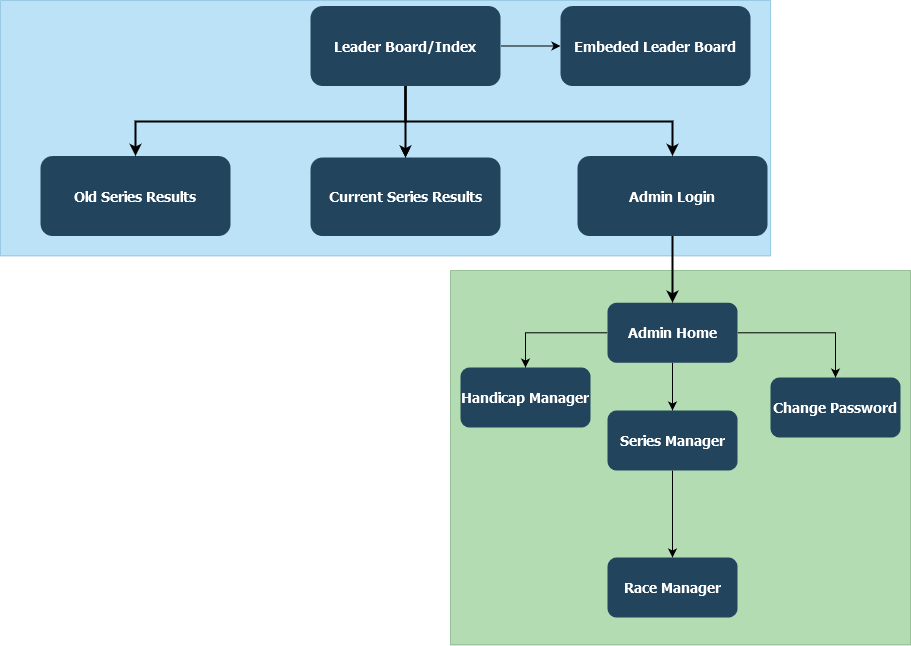
\includegraphics[width=1\linewidth]{images/SiteMap.png} 

    \caption{Site map showing the different pages of the web-app. The coloured boxes clearly show the two different sections of the website.
    }

    % use the notation fig:name to cross reference a figure
    \label{fig:Site Map}
\end{figure}

\subsection{Non-Admin Section}

\hfill\\
\subsubsection{Leader-board/index page}
\hfill\\
The first page a user sees upon opening the web-app is the leader-board page. This shows a summary of the ongoing series, and lists past series. Figure \ref{fig:LeaderBoardWF} is a wire-frame, showing the design of the page.

\begin{figure}[H]
    \centering
    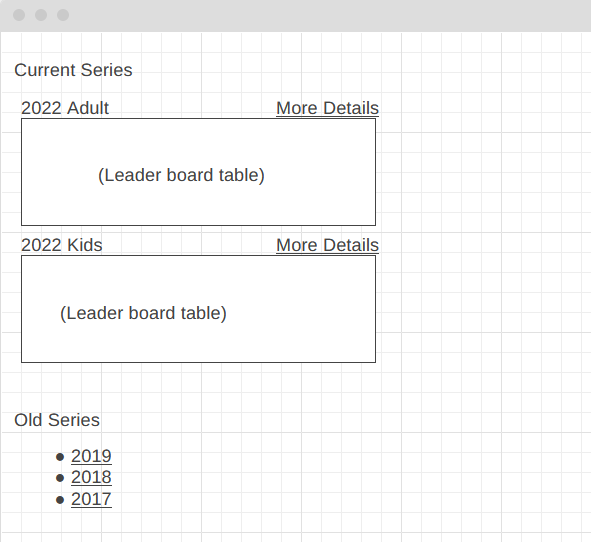
\includegraphics[width=1\linewidth]{images/IndexWireframe.png} 

    \caption{A wire-frame, showing the possible design of the Leader Board page.
    }

    % use the notation fig:name to cross reference a figure
    \label{fig:LeaderBoardWF}
\end{figure}


Series with the competed flag set to false in the database, representing the series that sailors are currently competing in, are displayed first. The leader-board for each series is shown with them.
\begin{itemize}
    \item
    There can be any number of series, as a club may have multiple happening simultaneously, but it is assumed there will be few of them, and so they can all be displayed properly on the same page
    \item
    The total score for each sailor in the Leader-board is not stored in the database, but is calculated from all the scores of all the races in the series. Although this results in more repeated computation on the sever, it removes the possibility of miss-matches between the total score shown and the real score, making adding and updating scores simpler.
    \item
    Each entry contains a link to a results page, showing more detail about the results of the races, including the results of individual races.
\end{itemize}
    
The next section of the page shows the series that have been completed, and a winner declared. The results for these are not as important, so they are hidden separate pages, assessed via links displayed on this page. This reduces clutter while still keeping the information easily accessible to users.

\hfill\\
\subsubsection{Current and old Series results pages}
\hfill\\
These pages show more detail about a specific series. They show the overall series leader-board, and a table for each race that race’s results. Figure \ref{fig:detailsWF} is a wire-frame showing the design:

\begin{figure}[h!]
    \centering
    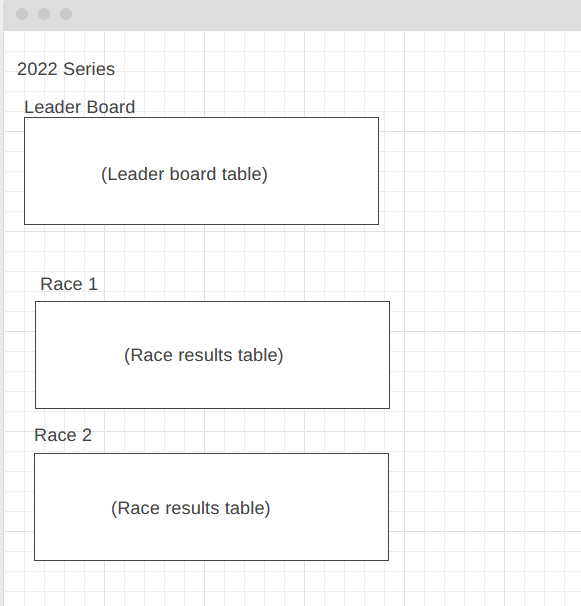
\includegraphics[width=1\linewidth]{images/moreDetailWireframe.png} 

    \caption{A wire-frame, showing the possible design, the current and old series results page.
    }

    % use the notation fig:name to cross reference a figure
    \label{fig:detailsWF}
\end{figure}

\hfill\\
\subsubsection{Embedded Leader-board}
\hfill\\
This page was not in the original design, but was added in later to fulfil the requirement in the could have section of the user stories that: “A user can embed the leader board of a series in another website to share results easier”. The page simply displays the leader-board of a given series, and a user can link this page in their own website to embed the leader-board in it.

\hfill\\
\subsubsection{Admin Login}
\hfill\\
The admin login page is a simple, generic login page that allows the admin user to log in to the admin account, in order to access to admin part of the website. Only a password is required, as there is only one admin account. This was done to reduce the complexity of managing accounts. This account is to be shared amongst all the people at the club responsible for inputting race data, similar to how currently, the single computer with the \citet{sailwave} program is shared.

\subsection{Admin Section}

\hfill\\
\subsubsection{Admin Home}
\hfill\\
This page features a list of all the series as links, split into current and past. Each series links to the series manager page for that series. The user can also use this page to add a new series. The page also contains links to the handicap manager and the change password page. A wire frame of the page is shown in figure \ref{fig:adminHomeWF}.

\begin{figure}[H]
    \centering
    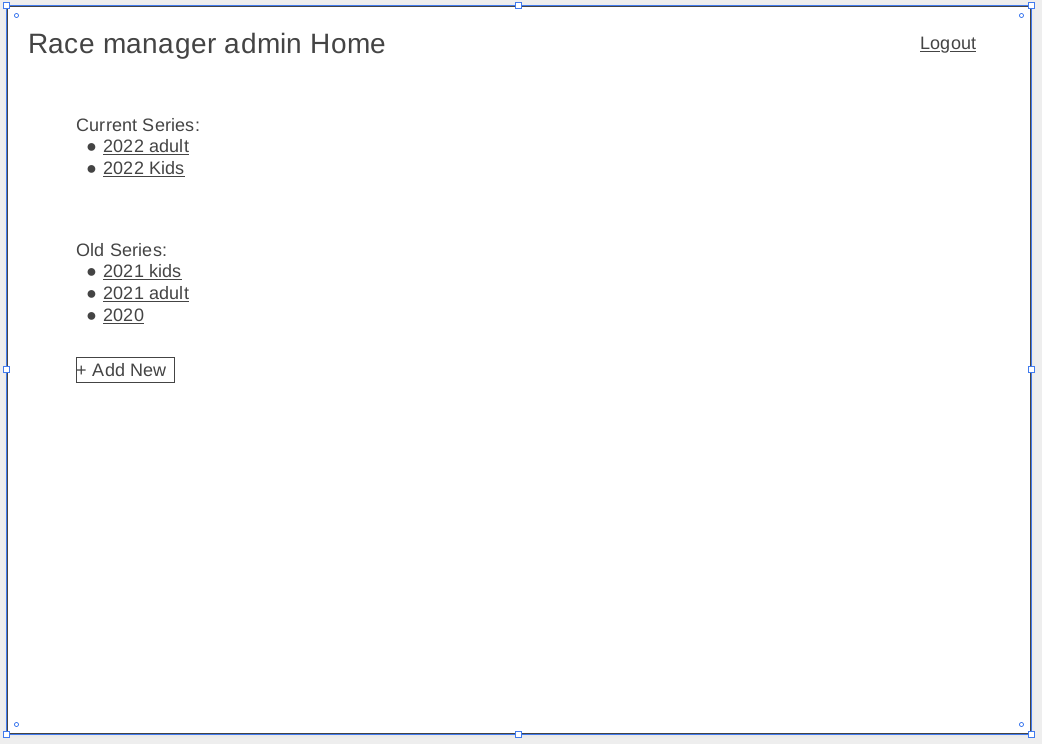
\includegraphics[width=1\linewidth]{images/admin home 2.png} 

    \caption{A wire-frame, showing the possible design of the admin home page.
    }

    % use the notation fig:name to cross reference a figure
    \label{fig:adminHomeWF}
\end{figure}

\hfill\\
\subsubsection{Handicap Manager}
\hfill\\
The handicap manager allows the user to manage a global list of boats and their handicaps. The Portsmouth Yardstick handicap numbers are only available on the RYA website in PDF format. This means that having a system to automatically import the handicap numbers from a file is not feasible, as this is hard to do with a PDF file. Additionally, any solution that did so would be reliant on the format of the Portsmouth Yardstick handicap numbers remaining unchanged.

The best solution that was found was to provide a way for the user to input and update handicap information manually. This also provides the benefit of allowing boats to be used that do not feature in the main Portsmouth Yardstick Scheme. This increases the web-apps flexibility.

The page will consist of an editable table, showing all the boats and handicap numbers currently in the system, with the ability to add more. The software will be delivered to the client with the most up-to-date handicap numbers preinstalled, so less setup is required. It will be up to the client to update these numbers when new ones are released by the RYA.

\hfill\\
\subsubsection{Change Password}
\hfill\\
This page will feature a simple form allowing the admin user to change the admin password.

\hfill\\
\subsubsection{Series Manager}
\hfill\\
The series manager page allows Admin users to edit a series. This includes adding new races, sailors, editing the parameters such as the penalty scores and the discount ratio and deleting the series. The page will also feature the leader-board for the series, so the user can see the effect of any changes they make. The wire-frame for the page is shown in figure \ref{fig:seriesEditorWF}.

The main features of the page are a couple of editable tables that can be used to add and edit the details of races and sailors. The parameters can be tweaked via a series of options at the top of the page, For example, the completed checkbox in the wire-frame.

\begin{figure}[H]
    \centering
    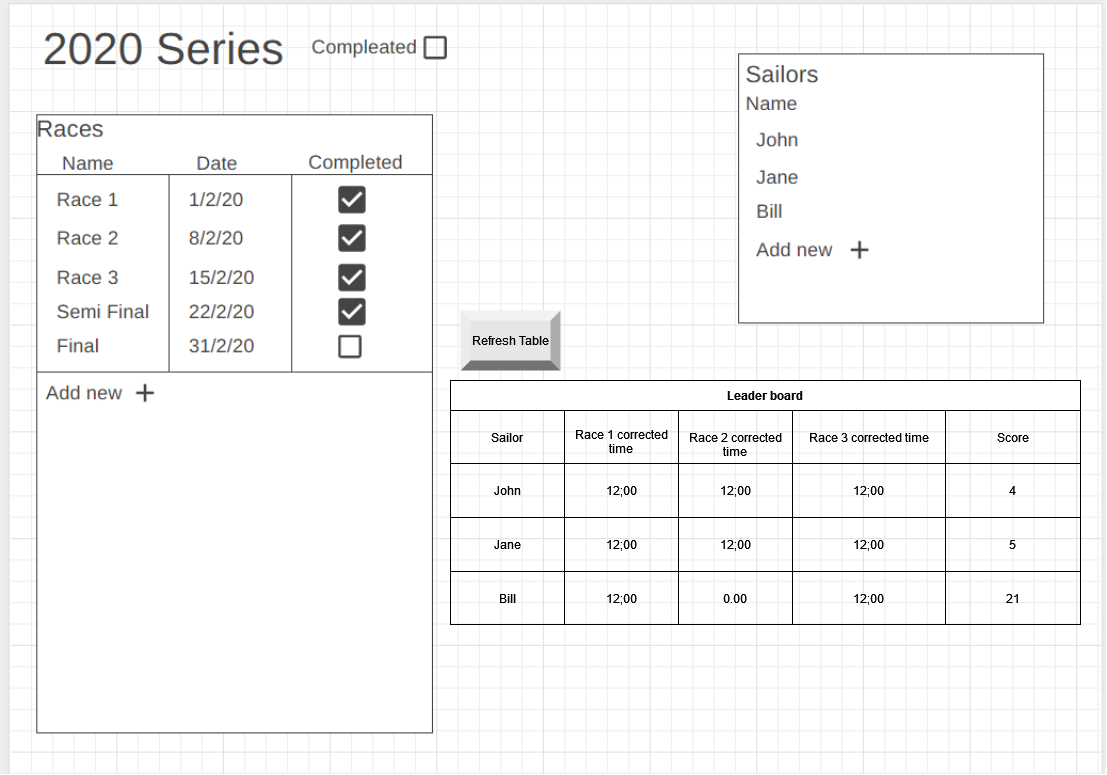
\includegraphics[width=1\linewidth]{images/Series editor 2.png} 

    \caption{A wire-frame, showing a possible design of the series editor page.
    }

    % use the notation fig:name to cross reference a figure
    \label{fig:seriesEditorWF}
\end{figure}

\hfill\\
\subsubsection{Race Manager}
\hfill\\
By clicking on each race, the user is able to open up the race manager page for that race. This is the page where the results for a single race can be entered. Figure \ref{fig:raceEditorWF} is a wire-frame showing a possible design of the race table.

\begin{figure}[h!]
    \centering
    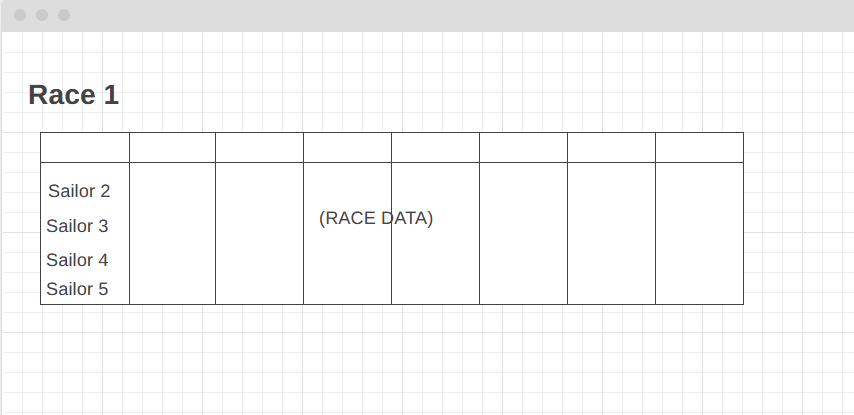
\includegraphics[width=1\linewidth]{images/Race editor.png} 

    \caption{A wire-frame, showing a possible design of the race editor page.
    }

    % use the notation fig:name to cross reference a figure
    \label{fig:raceEditorWF}
\end{figure}

The page mainly features an editable table showing all the race entries for that race. A race entry is a sailor in a race. The fields in the table allow all the database attributes for the Race Entry table to be edited. Unlike the tables on the previous page, the user cannot add new entries manually. Whenever a new race or sailor is added in the series editor, new entries are automatically added to the race entry table. This ensures that there is always a race entry for every sailor in every race. In this way, when a new sailor is added to a series, they are automatically entered into every race in that series. This reduces the workload of the admin user, and ensures that any sailor who didn't complete in a race are counted as not competing, as that is the default state of a sailor when they are added.

\section{Scoring}

In order to meet the requirements, the web-app must currently process the race data entered by the user into scores.

There are two scores which must be managed, the score for each sailor in a race, and a sailor's total score across a series. One approach would be to store these scores in the Race Entry and Series tables respectively, and update them whenever something changes. However, it was decided that a better approach would be to only calculate the scores when they are needed. While this increases the processing needing to be done on the server, it removes the chance for a mismatch between stored score data, and the inputs. It also reduces the complexity of updating the database, and reduces all the score processing into one algorithm, making it easier to find bugs in it, as there is only a single point of failure.

Formula \ref{eq:1} shown in chapter \ref{chap:Back} will be used to calculate the corrected time from the raw time, whenever an attribute in the Race entry table is updated. When a user loads the Leader Board table, and requests the info from the server, the list of race entries for each race in that series will be sorted by corrected time, and the score for each sailor is calculated via the RYA low scoring race rules \citep{RYAscore}, with penalty scores being awarded where the relevant attributes are set. The scores for every sailor in the series will then be added together, and sorted. They can then be sent to the client-side to be displayed.

In this way, scoring should follow the RYA scoring rules \citep{RYAscore}.

\section{Validation}

The system will be designed to handle as much validation as possible in the database itself so, theoretically, the database cannot be in an invalid state. This means data from the database can be trusted, and so removes the need for extensive validation on data received from the database.

From the point of view of inputting data, where possible, the user will be prevented from entering incorrect data at all. For example, in fields such as time, there only numeric values are valid, the user will not be able to enter non-numeric values at all. This removes the need for lots of validation messages which, especially on a large table with many editable fields that the user may be filling in, could get overwhelming.

\section{Communication with the Database}

The majority of communication with the database will be done on the server-side upon the receipt of a GET for POST request. However, on the pages with editable tables, such as the race editor and Series editor, a different approach is required. In order to avoid having to reload the page every time data in the table is changed by the user, which would be very annoying and may make the site unusable, asynchronous communication with the server in needed. The new data must be sent in a POST request to the server, without reloading the page. From there, the server will update the database.

\section{Conclusion}

Overall, the web-app is designed to be simplistic, and to not crowd pages with too many features, as was the main issue in \citet{sailwave}. The design should meet the requirements, while keeping the interface easy to grasp by non computer skilled users.


%==================================================================================================================================
\chapter{Implementation}\label{chap:imp}
What did you do to implement this idea, and what technical achievements did you make?
\section{Technologies}

\subsection{The Django framework}
This project was developed using the Django web-app framework. This section will explain the Django framework, and discuss why it was chosen

The website for the Django Framework \citep{django} say that Django is a high level framework that encourages rapid development and clean design. From researching on this website, the advantages and disadvantages of using Django are as follows:

Advantages:
\begin{itemize}
    \item 
    Django is a Full-stack framework, which means that everything is included. e.g. database, admin interface, templates etc.
    \item 
    The Built-in Database framework means no need to write SQL or host a separate database.
    \item 
    Django is optimised for fast development.
    \item 
    Developer has experience with Django.
\end{itemize}
Disadvantages:
\begin{itemize}
    \item 
    Slower than flask to get the basics set-up.
    \item 
    It is less flexible, as everything is built-in.
    \item 
    Features are a bit overkill for small, simple apps, such as this project is likely to be.
\end{itemize}

The other choice of framework for this project is Flask. According to its website \citep{flask}, flask is a lightweight web application framework, designed to make getting started quick and easy. Flask doesn't enforce dependencies for project layout, and it is up to developers to choose the tools they wish to use. The advantages and disadvantages of using flask are as follows:

Advantages
\begin{itemize}
    \item 
    More flexible as the developer can pick and choose the libraries and tools to use.   
    \item
    As it is lighter weight, it allows for a more easy installation and setup.
\end{itemize}
Disadvantages
\begin{itemize}
    \item 
    Has fewer features built-in.
    \item 
    developer must learn it from scratch, as no past experience.  
    \item 
    less scaleable. Mostly recommended for small web-apps.
\end{itemize}

Overall, the clear choice appears to be Django. The two frameworks are remarkably similar and seem to do things in very similar ways, and the simple advantage that less time is needed to learn the framework with Django due to experience is a clear advantage.

Another clear advantage is that because Django is a higher-level framework than flask, it allows for a faster development time, meaning more effort can be put into creating a better product, rather than doing the creating.

In terms of flask, the flexibility advantage does not help much in this project. A sailing race manager is at its core a simple app to store data in a database, retrieve it and process, and so is the exact problem Django seems to have been designed for. Therefore, the flexibility of being able to do more different things with the framework is not particularly useful.

In conclusion, Django appears to have several clear advantages over flask, with the advantages of flask not being that relevant to this project. 

\subsection{Development Environment and deployment}

A variety of tools were used to develop and deploy this project. First, a virtual environment was used in developers using venv. The python doc page on venv \citep{venv} explains the need for a virtual environment and how it works. Venv specifically was chosen as it is easy to set up and works with python, which Django is a library of.

In order to deploy the project, the code was gathered into a docker container for easy deployment, that being one of the goals of the project. The resulting docker container was hosted for testing using Amazon Web Services (AWS). The resources required remained in the AWS free tier, meaning no cost was occurred when hosing the Web-app publicly, for the client to look at.

\subsection{The SQLite Database Engine}
Django supports multiple database engines, but the built-in SQLite is, in this case, the best option. A page on the website for SQLite, describes what it is and what it is suitable for \citep{SQL}.

SQLite requires no administration, and so would make it easier for sailing club people to maintain it. It does not require a separate server, making it much easier to be deployed by inexperienced people in few steps. The website says it works well with standalone small websites and applications.

The downside is that it has little security and it not scaleable. Low security doesn't matter as the data stored in it by individual small clubs is not particular sensitive, and scaleability does not matter as the web app is designed to be used by individual small scale clubs, and is very unlikely to hit the limit stated on the website of 100k hits/day.

Also, SQLite does not have strong concurrency mechanisms. This is not an issue as the web app is designed, so very few people should be editing the database at any one time.

\subsection{The Jspreedsheet JavaScript library}

A spreadsheet-like interface, similar to that currently used in \citet{sailwave}, was one of the requirements for this project. To achieve this, the JavaScript Library, Jspreedsheet \citeyear{Jspreadsheet} was used. It allows fully functional spreadsheets to be added to HTML pages. All the tables on the web-app were made using this library.    

\section{Development Straragy}  

\subsection{The Agile Methodology}

An agile mythology was followed when developing this project. This helps deal with uncertainty in the requirements, and allows working prototypes to be produced quickly, so the requirements could be refined \citep{agile}. It also ensured development presided rapidly, which was essential due to the limited resources of one developer and the strict deadline that this project had.

The developing work was split up into "sprints". Each sprint covered, approximately, a different feature. After an initial planning phase which included the initial meeting with the client, the sprints presided as below: 
\begin{enumerate}
    \item
    Environment Setup
    \item
    Database
    \item
    Leader board page
    \item
    Admin login and series viewer
    \item
    Series editor
    \item
    Race editor
    \item
    Client meeting and modifications
    \item
    Bugfixes and cleaning up and additional modifications from client
    \item
    Delivery
\end{enumerate}
\hfill\\
In the classic agile methodology, the client is involved heavily in the project and feedback is obtained, ideally after every sprint \citep{agile}. This was not possible in this project because, as described in the Introduction, the client was not able to dedicate much time to the project. Because of this, feedback could only be obtained towards the end of development, when a working prototype had been produced. A meeting was held in February 2023 with the client, and several shortcomings were identified, as described in the next section. Written feedback was obtained twice more in the following weeks, and a final evaluation of the project was given by the client at the very end of the project. 

\subsection{Evolution of Requirements}

Due to the inability to obtain frequent feedback from the client, the requirements remained the same until the second meeting towards the end of the project. At this meeting, a number of issues were raised. They are summarised below:
\begin{itemize}
    \item 
    The handicap numbers were not shown when adding race results, the client wanted this, so it was more clear that the handicap system worked.
    \item
    The client wanted non-admin users to be able to see more information about individual races, like raw times, points per race and corrected times, not just the Series leader board with the overall points.
    \item
    The client wanted the discount feature to be implemented, as it had not been yet.
    \item
    The client desired on obvious reload button on the leader boards, so users could be sure they were viewing the most up-to-date information.
    \item
    The client wanted the user to be able to set custom did not finish and score officer scores for each series.
    \item
    The scores were being incorrectly calculated, due to a misunderstanding of the requirements, the corrected time was being treated as the score, instead of the score being awarded by finishing place of participants.
\end{itemize}

The requirements were amended to accommodate these changes and mistakes. Feedback was sought twice more, with a number of smaller issues being identified and fixed. A few issues were never successfully addressed. These will be explained in chapter \ref{chap:eval}.


\subsection{Testing and Documentation Strategies}

Unit testing is widely considered an essential part of software development, and can save huge amounts of debuting and integration time \citep{unittest}. In this project, an attempt was made to follow a strategy of test wiring, to ensure tests were kept extensive and up to date. Towards the end of the project, the strategy broke down and had to be abandoned.

First, we will describe the testing strategy that was used. Django uses a model-view-template architecture \citep{django}. These three parts of the Django app all need to be tested. The Django docs \citep{django} were used as unit tests were developed for the project.

To test the model or database, unit tests were used to test valid and invalid data inputs, to make sure the database accepts correct data, and rejects incorrect data. Boundary data was not tested, as there are not many parts of the database where this would particularly apply. Leavening these out significantly deceases the amount of tests that need to be written. Testing that the database accepts correct data types has been left out as Data types are enforced in the database, so these tests were more testing Django's database code than my own, which is a waste of time. We can also assume, due to the design of only letting the user input valid data, that any data that reaches the database is of the correct data type.


In terms of views, which in Django is the backend code that handles requests to the web-app, this logic was tested to make sure it works, and returns a context dictionary with the correct content for the HTML pages to display.

Testing templates is more complex. Django has a built-in template engine, which allows HTML pages to inherit from each other \citep{django}. Because this web-app is small in scale, it is not worth it to implement automatic testing of the template, as this is a complex task and can require special tools to accomplish. The best solution is to test the template manually to see if the UI elements show up correctly.

The strategy for writing the tests was, at the end of every sprint, to write unit tests covering the features implemented in that sprint. At the same time, the tests themselves and how the feature was implemented was to be documented. As the project progressed, it became apparent that writing tests and documentation was drastically slowing down development speed. Around January 2023 it was decided that the project would not be completed if the current strategy continued to be followed. It was decided to stop testing and documentation, and focus only on development of features, in order to ensure all the requirements were met in time for the deadline in March. The need for documentation and unit tests was not so great as in other projects, due to the fact that this project only has one developer. This means that detailed documentation and testing is not as necessary during development, as there is no need for others to understand the code at that time. Because of this, it was deemed a necessary sacrifice.

The result was that, by the end of the project, the web-app had very poor documentation and unit test. This was made worse by the fact that much of the testing and documentation that was written early in the project was no longer valid due to changes in requirements and design. However, the project had successfully implemented the requirements.

\section{Explanation of Implementation}
In this section, we will look at how various problems were solved when implementing the design, and how each part of the web-app works.

\subsection{Model/Database}

The built-in Django database engine makes building a database very simple. The structure of the database is specified in a python class, and Django handles everything else. The only issues involved were dealing with multiple objects with the same name, and validation.

As per the design, as much validation as possible was done in the database. Field data types were strict, and a cascade rule was implemented meaning when an abject in the database was destroyed, all objects associated with it are also destroyed. This ensues that the database is always in a valid state, and there are no references to non-existing objects.

The calculation of corrected time was also done in the database. a custom save method was used so whenever a race entry is added or updated, the corrected time is calculated and stored in the database. This means that the corrected time is always up-to-date. Null values in the Race Entry table had to be handled, so corrected time was only calculated when all the data required for the calculation was available.

It was decided to allow the user to input any number of sailors and races with the same name. This means validation checking if a name already exists was not needed. However, a way to distinguish different objects with the same name was still needed, in order to display the Series and Race Editor pages that dealt with these objects. The solution was to rely on the URL slug, that was needed when the names appeared in URLs, to distinguish objects. An algorithm was implemented that ensured that all slugs were different, even if the name of some of the objects were the same. It did this by appending numbers to the object's slug if the slug already existed in the database.
 
\subsection{View/Backend}

The main issues that had to be dealt with in the backend were providing data in the correct format for the JavaScript tables to understand, and dealing with asynchronous requests.

The backend is written in python, and so when data from this is passed to the template, that data is in a python format. Because the tables on the pages were written in JavaScript, a way was needed to translate data between the two languages. The solution that was used was to convert the data into Json data format, using libraries built into python and JavaScript, before sending it to the client (as in client-server architecture), and then converting it into a JavaScript list once it arrives, in order to feed it to the tables. This worked well, apart from when the data contained boolean values. Because, python represents boolean value as "True/False" and JavaScript represents them as "true/false", JavaScript would not recognise them as boolean values. This means that these had to be manually converted from Json to JavaScript.

The design required that the webpages did not reload every time a value in a table was updated. This meant asynchronous communication was needed in order to pass changes to the database. this was achieved using AJAX and jQuery. These are two popular JavaScript libraries, that allow requests to be sent from the client to the server without reloading the page the client is viewing. jQuery contains wrapper functions that make working with AJAX easier to do. When a post request is received by the server, a "command" value tells the server what to do. A large if-else statements dealt with all the possible values of "command".

\subsection{Template/Client-side}

The main complexity on the client side comes with using the Jspreadsheet library to display the tables. It became apparent, as development proceeded, that Jspreadsheet was not the most suitable library to use, and its documentation was at times poor. However, it was too late to change to a different library for tables. Jspreadsheet is designed to make interactive spreadsheets. What this project required, was closer to HTML tables than a spreadsheet, so lots of functionality, like keyboard shortcuts to add new cells, rearranging cells and deleting them, had to be removed. This resulted in quite messy code.

The Jspreadsheet library included event handlers for when cells are selected or updated. These were used to call functions when the value in the cell had been changed by the user, that sent AJAX requests to the server to update the database accordingly. In this was, that tables on the client side and the database were kept in identical states. This was only true for tables where the user can edit them. For the others, e.g leader board and race summary tables, The user had to manly refresh the page using the required button. This was done to reduce the amount of Ajax requests, which reduces load on the server and the network. A user doesn't need to update the leader board tables as much as they edit values, so the refreshing of the page was not too much of an issue.

In order to identify which record in the database to change when the user inputs data, the following approach was used. The order that data is displayed in tables on the client-side is the same order as it is stored in the database. In this way, row 1 in a table on the client side corresponds to row 1 in the database. The X Y position on an updated item in a table con the client side is sent to the server in the AJAX request, so the server knows which value to update. This solution was simple when there were few tables, but as the tables in the web-app got more complex, it resulted in some complex and fragile code. It also meant that users cannot sort tables in which they input data, as challenging the order that the data in displayed would mean the wrong data in the database is updated. A better solution would be to store the primary key for each object in the database in a hidden column, in its corresponding row in the client-side table. This would mean that the correct object could be accessed directly from the database. This was not implemented, as there was no time to do the significant code refactoring that would be required for this to work.


%==================================================================================================================================
\chapter{Evaluation}\label{chap:eval}
In order to evaluate how well the project met the requirements, the client was asked for some formal feedback, and a survey was conducted to gather the opinions of the members of Castle Semple Sailing Club, as well those of a few others involved in dingy sailing outside the club.

\section{Client feedback}

Final feedback from the client was given by Dr Simon Rogers. His full response is quoted below:

\begin{displayquote}
    \begin{outline}
        \1 
        From my inspection, the app meets all essential requirements.
        \1
        (with a data hat on) The backend database structures are sensible, and well thought out.
        \1
        I don't know what js library you're using for the various tables, but it seems a bit buggy for me (using firefox). I.e. I've noticed two bits of weirdness:
            \2 
            when I click the drop down to select a boat, nothing happens. Although if I press a key in the box the list appears (although the list doesn't filter based on the key I pressed)
            \2
            sorting columns seems to work sometimes, with a delay
        perhaps they're just slow as it's having to do some backend lookups? In which case, some kind of cache would be useful.
        \1 
        There's a bug in the view races button. This shows up for the 2022 series -- looks like a string is being added to an int somewhere -- probably a very easy fix.
        \1 
        One of the proposed output tables has never been developed. In particular, in the leaderboard table, the user can see times for each race and total points for the series, but not the original request: a choice of uncorrected times and/or corrected times and/or points (all per race) and total series points. IMO this makes the table hard to interpret. Not sure why not just have three columns per race with that info in? I guess this wasn't formally a requirement, but was discussed a couple of times and I think makes uptake of the app less likely. At the very least, it should be really clear that the times in the series table are corrected, the headings don't make this clear.
        \1 
        Navigation through the pages is easy, although some help text in various places would be useful. E.g. to explain to the user what to do -- just a few sentences here and there. I'm not sure a non-computer-savvy user would be able to work things out quickly by themselves. A few sentences on each page and they'd be sorted though. e.g. "To add a new race, click blah and then blah etc...once you've finished mark a race as complete and it will be included in calculations blah blah".
        \1 
        minor, but my guess is that you've built a single type of user (admin) -- admin can make all changes, everyone else just views. Fine, I guess, but probably would be neater to add an extra layer inbetween that can do all the editing, leaving admin as someone who can really screw things up! Also, >1 person might be entering, and wouldn't be great for them to all access via the same account.
        \1 
        Also minor. The table formatting -- would be good to be able to see more quickly which columns mean which things. I.e. first column is sailor, last is points total, and the others are races. Perhaps some nested headings would have worked well here, or using shading.
    \end{outline}
\end{displayquote}

The feedback is summarised and collected into categories in the table below. The fourth point from the initial feedback was not included, as that bug was fixed prior to sending out the questionnaire.     

\begin{table}[H]
    \centering
    \caption{Issues raised by participants ion the survey, grouped into categories}
    \begin{tabular}{|l|p{0.8\linewidth}|}
    \hline
        \textbf{Categories} & \textbf{Issues}  \\ \hline
        \textit{Bugs} & drop down menu sometimes doesn't respond.   \\ \hline
        ~ & delay in sorting columns \\ \hline
        ~ & ~ \\ \hline
        \textit{Lack of information on tables} & leader board table doesn't contain enough information.   \\ \hline
        ~ & \\ ~ \\ \hline
        \textit{Lack of instruction} & column headings are not clear on some tables.  \\ \hline
        ~ & lack of help text + instructions on the website. \\ \hline
        ~ & \\ ~ \\ \hline
        \textit{issues with features} & one admin account that can do everything is not good \\ \hline
    \end{tabular}
    \label{tab:table client feedback}
\end{table}

\section{Questionnaire}

To get a better idea of the extent to which this project has satisfied the requirements, a questionnaire was made and sent out to the members of Castle Semple Sailing Club. It was unfortunately not possible for many of the members to provide feedback, so the questionnaire was entered to other people outside the club, who have an involvement in dingy sailing. The full questionnaire is available in appendix \ref{apend:questions}.

The questionnaire is split into three sections. One for the non-admin functionality of viewing results, one for the Series Editor, and one for the Race Editor. In each section, the participants were asked to rate how clear and useable the section was overall out of 5, with 1 being not unclear and unusable and 5 being very clear and usable. They were also asked for any issues they had with the section, and anything the section was missing. These last two were asked as open-ended textual responses.

At the start and end of the questionnaire, participants were informed what the collected data was being used for, and that they could withdraw their consent at any time. All data was collected anonymously.

\section{Results}

\subsection{Non-Admin Section}
A graph showing how the participants rated the clarity and usability of the non-admin section of the website is shown in figure \ref{fig:results1}

\begin{figure}[H]
    \centering
    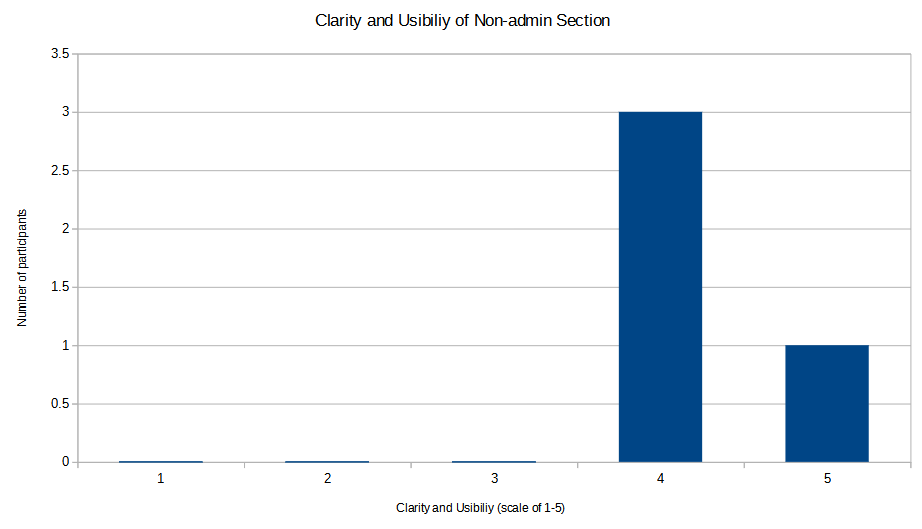
\includegraphics[width=1\linewidth]{images/Results 1.png} 

    \caption{A graph showing how participants rates the clarity and usability of the Non-Admin section of the web-app, on a scale of 1-5.
    }

    % use the notation fig:name to cross reference a figure
    \label{fig:results1}
\end{figure}

The responses for issues participants had with the section are given in table \ref{tab:table 1}, grouped into categories.

\begin{table}[!ht]
    \centering
    \caption{Issues raised by participants ion the survey, grouped into categories}
    \begin{tabular}{|l|l|l|l|l|l|l|l|l|l|}
    \hline
        \textbf{Categories} & \textbf{Responses}  \\ \hline
        \textit{Presentation and Colour} & grey type is a bit faint to read  \\ \hline
        ~ & Some colour differentiation would be good  \\ \hline
        ~ & ~ \\ \hline
        \textit{Issues with functionality} & Some of the table functionality seems to hang  \\ \hline
    \end{tabular}
    \label{tab:table 1}
\end{table}

The responses for things participants thought were missing from this section are shown in table \ref{tab:table 2}, grouped into categories.

\begin{table}[H]
    \centering
    \caption{Issues raised by participants ion the survey, grouped into categories}
    \begin{tabular}{|l|p{0.8\linewidth}|}
    \hline
        \textbf{Categories} & \textbf{Responses}  \\ \hline
        \textit{Presentation and Colour} & More distinctive colours for table header for easier viewing, however the page is legible regardless  \\ \hline
        ~ & ~ \\ \hline
        \textit{Lack of information} & There is no space for sail number or crew to be displayed, which is information some people might like to see  \\ \hline
        ~ & Inclusion of more information in the tables would make it more usable -- uncorrected times, corrected times, and points for each race.  \\ \hline
    \end{tabular}
    \label{tab:table 1a}
\end{table}

\subsection{Series Editor}
A graph showing how the participants rated the clarity and usability of the Series Editor of the website is shown in figure \ref{fig:results2}

\begin{figure}[H]
    \centering
    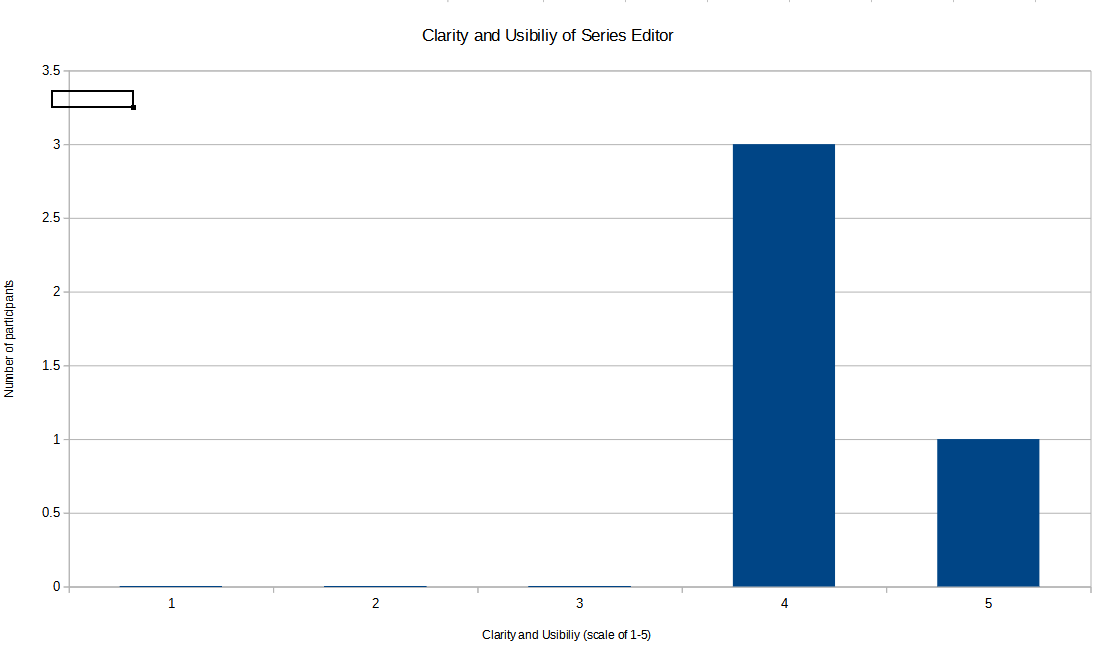
\includegraphics[width=1\linewidth]{images/results 2.png} 

    \caption{A graph showing how participants rates the clarity and usability of the Series Editor, on a scale of 1-5.
    }

    % use the notation fig:name to cross reference a figure
    \label{fig:results2}
\end{figure}

There were no responses for the question do the participants have any issues with the Series Editor

The responses for things participants thought were missing from this section are shown in table \ref{tab:table 2}, grouped into categories.

\begin{table}[H]
    \centering
    \caption{Issues raised by participants ion the survey, grouped into categories}
    \begin{tabular}{|l|p{0.8\linewidth}|}
    \hline
        \textbf{Categories} & \textbf{Responses}  \\ \hline
        \textit{Lack of information} & It would be useful to see positions as well as times in the results section. For larger fleets it's not always immediately obvious where someone's time sits in the grand scheme of things.  \\ \hline
    \end{tabular}
    \label{tab:table 2}
\end{table}

\subsection{Race Editor}
A graph showing how the participants rated the clarity and usability of the Race editor of the website is shown in figure \ref{fig:results3}

\begin{figure}[H]
    \centering
    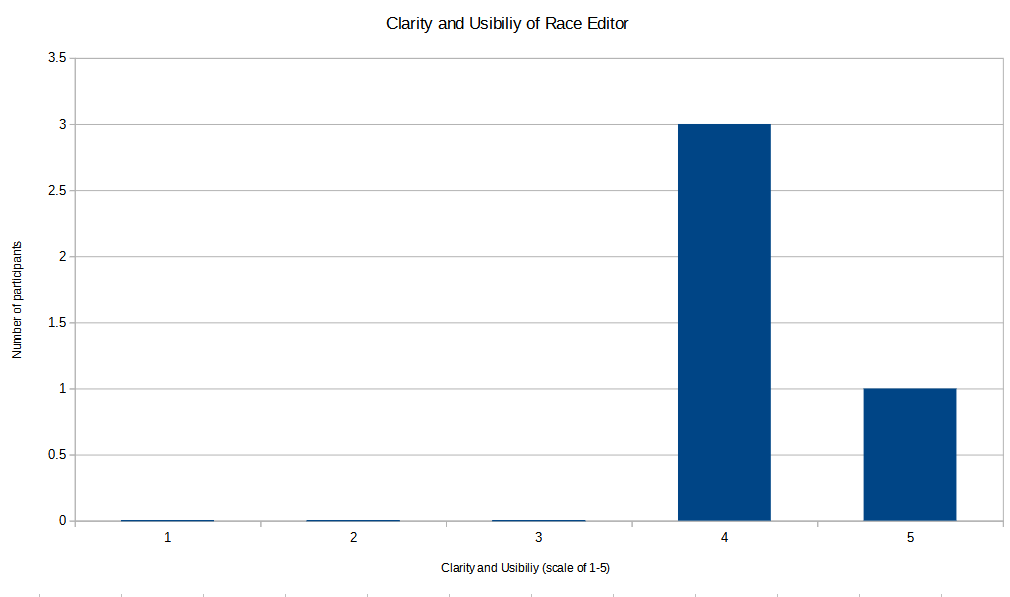
\includegraphics[width=1\linewidth]{images/Results 3.png} 

    \caption{A graph showing how participants rates the clarity and usability of the Race Editor, on a scale of 1-5.
    }

    % use the notation fig:name to cross reference a figure
    \label{fig:results3}
\end{figure}

The responses for issues participants had with the section are given in table \ref{tab:table 1}, grouped into categories.

\begin{table}[!ht]
    \centering
    \caption{Issues raised by participants ion the survey, grouped into categories}
    \begin{tabular}{|l|p{0.8\linewidth}|}
    \hline
        \textbf{Categories} & \textbf{Responses}  \\ \hline
        \textit{Presentation and Colour} & why is some type black and some grey?  \\ \hline
        ~ & ~ \\ \hline
        \textit{Issues with functionality} & Boat dropdown doesn't always work, although dropdown appears if I type into the box  \\ \hline
    \end{tabular}
    \label{tab:table 3}
\end{table}

There were no responses for what participants thought was missing from the race editor.


\section{Analysis of Results}

The final feedback from the client makes it clear that the web-app, in general, meets the requirements of the project. The issues raised from the feedback can be collected into categories, as shown in table \ref{tab:table client feedback}. 

In the feedback, the customer states that many of these are minor. However, they nevertheless affect the usefulness of the final product. The client picked up on some bugs, which are inevitable given the lack of proper testing that the project went through. These should be able to be easily solved in any future maintenance updates, and the description of them as "minor" indicates that they do not harm the usability of the product significantly.

The client pointed out that the information given in the leader board tables is lacking somewhat. They desired original time and points to be shown along with the corrected time per race in the main leader board table, rather than it being hidden away behind the "view races" button. Due to the focus on keeping information very simple and readable in the design of this project, it appears that too much information has been hidden away, decreasing the usability of the final product. This issue had been previously brought up, but no way could be found to include all that information on one table and have it still easy to read.

Another system of the design focus to keep the web-app simple and minimal was a lack of help test anywhere in the program. The client picked up on this and indicated they would like some explanation around some of the harder to grasp features, such as what the completed checkbox on races does.

The final issue the client has is with the design choice to have only one admin account. This was done to limit the complexity of the account system on the web-app, which did allow for a more rapid development of the project. This turned out to be important, due to the lack of time towards the end of the project, which lead to thorough testing and documentation having to be dropped. However, it is true that the design took this strategy too far in this case, as one admin account raises many issues around security and concurrent use of the program. While in its current state, it is possible for multiple people to be signed in at once, it may cause problems that only more through testing that is possible would uncover.

Looking at the ratings participants gave the different sections of the web-app in the graphs in figures \ref{fig:results1}, \ref{fig:results2} and \ref{fig:results3} it is interesting to note the results for all the sections are that same. This was due to the low number of participants. The results are still useful, however, as they tell that the participants do find all parts of the website clear and usable. As the participants are Castle Semple Sailing Club members, and others of a similar demographic, this is evidence that the project was successful is its goal of creating a solution to the problem of a sailing race management system that is simple to use. The strength of the evidence is limited by the very low number of participants. A broader trial would be needed to obtain definitive evidence, but the results of such a trail are likely to follow those found here. This is due to the fact that the evidence from this questionnaire was so strongly in favour of the website being clear and usable.

The free text responses for all the sections in tables \ref{tab:table 1}, \ref{tab:table 1a}, \ref{tab:table 2} and \ref{tab:table 3} highlight similar issues to those the client gave in their final feedback. Mainly, the responses from the questionnaire inform that some improvements can be made to the presentation of the web-app, as well as again bringing up the issue of there not being enough information on the leader board.

Overall, it can be said that the evidence suggests that the final product of this project generally meets the requirements from the customer. It appears that the design choice of keeping the product clear and simple went too far in some areas, particularly the content of the leader board table, and the admin account system. These issues reduce the usability of the product, but they do not render the system unusable by the client.



%==================================================================================================================================
\chapter{Conclusion}

\section{Project Conclution}

This project set out to create a web-app to manage sailing races for Castle Semple Sailing Club. It aims to create a system that supported the RYA racing rules, and that could replace the system currently being used by the sailing club, Sailwave. A system has been successfully developed that meets the customer requirements, and is regarded by perspective users to be very clear and usable. The project used various tools to build this system on the Django web framework. 

The system was designed to function similarly to the Sailwave system, being a management program built around spreadsheet-like tables for data entry, designed to be used by one person at a time. The system also has an interface for anyone to view the results of races, similar to the Victoria Park Run website, and the whole thing is hosted on a web-app to allow for easy access.

The resulting product was deemed to successfully meet the client's requirements of a system that can replace the system they currently use. This was determined by detailed feedback from the client and a survey of prospective users. Several issues were identified with the final product that decrease its usability. Despite this, the overall system functions to the satisfaction of the customer, and it has solved the problem which this project set out to solve.

\section{Suggestions for the Future}

In order to improve the product of this project, work could be done to solve the issues the client had with it. The UI design of the system was kept basic, and most of the design went into the functionality. There is room for a more sophisticated UI to be implemented, which would increase the attractiveness of the web-app for sailing clubs. 

Additionally, there is the possibility of redesigning the web-app to make it more usable by different sailing clubs. This could be done by adding more features, to account for the differences in the way sailing clubs conduct races. The current solution is specially tailored to the needs of Castle Semple Sailing Club, and tweaks could be made to improve relevancy to other clubs.

%==================================================================================================================================
%
% 
%==================================================================================================================================
%  APPENDICES  

\begin{appendices}

\chapter{Appendices}
\pagenumbering{Roman}

\section{User Manual}
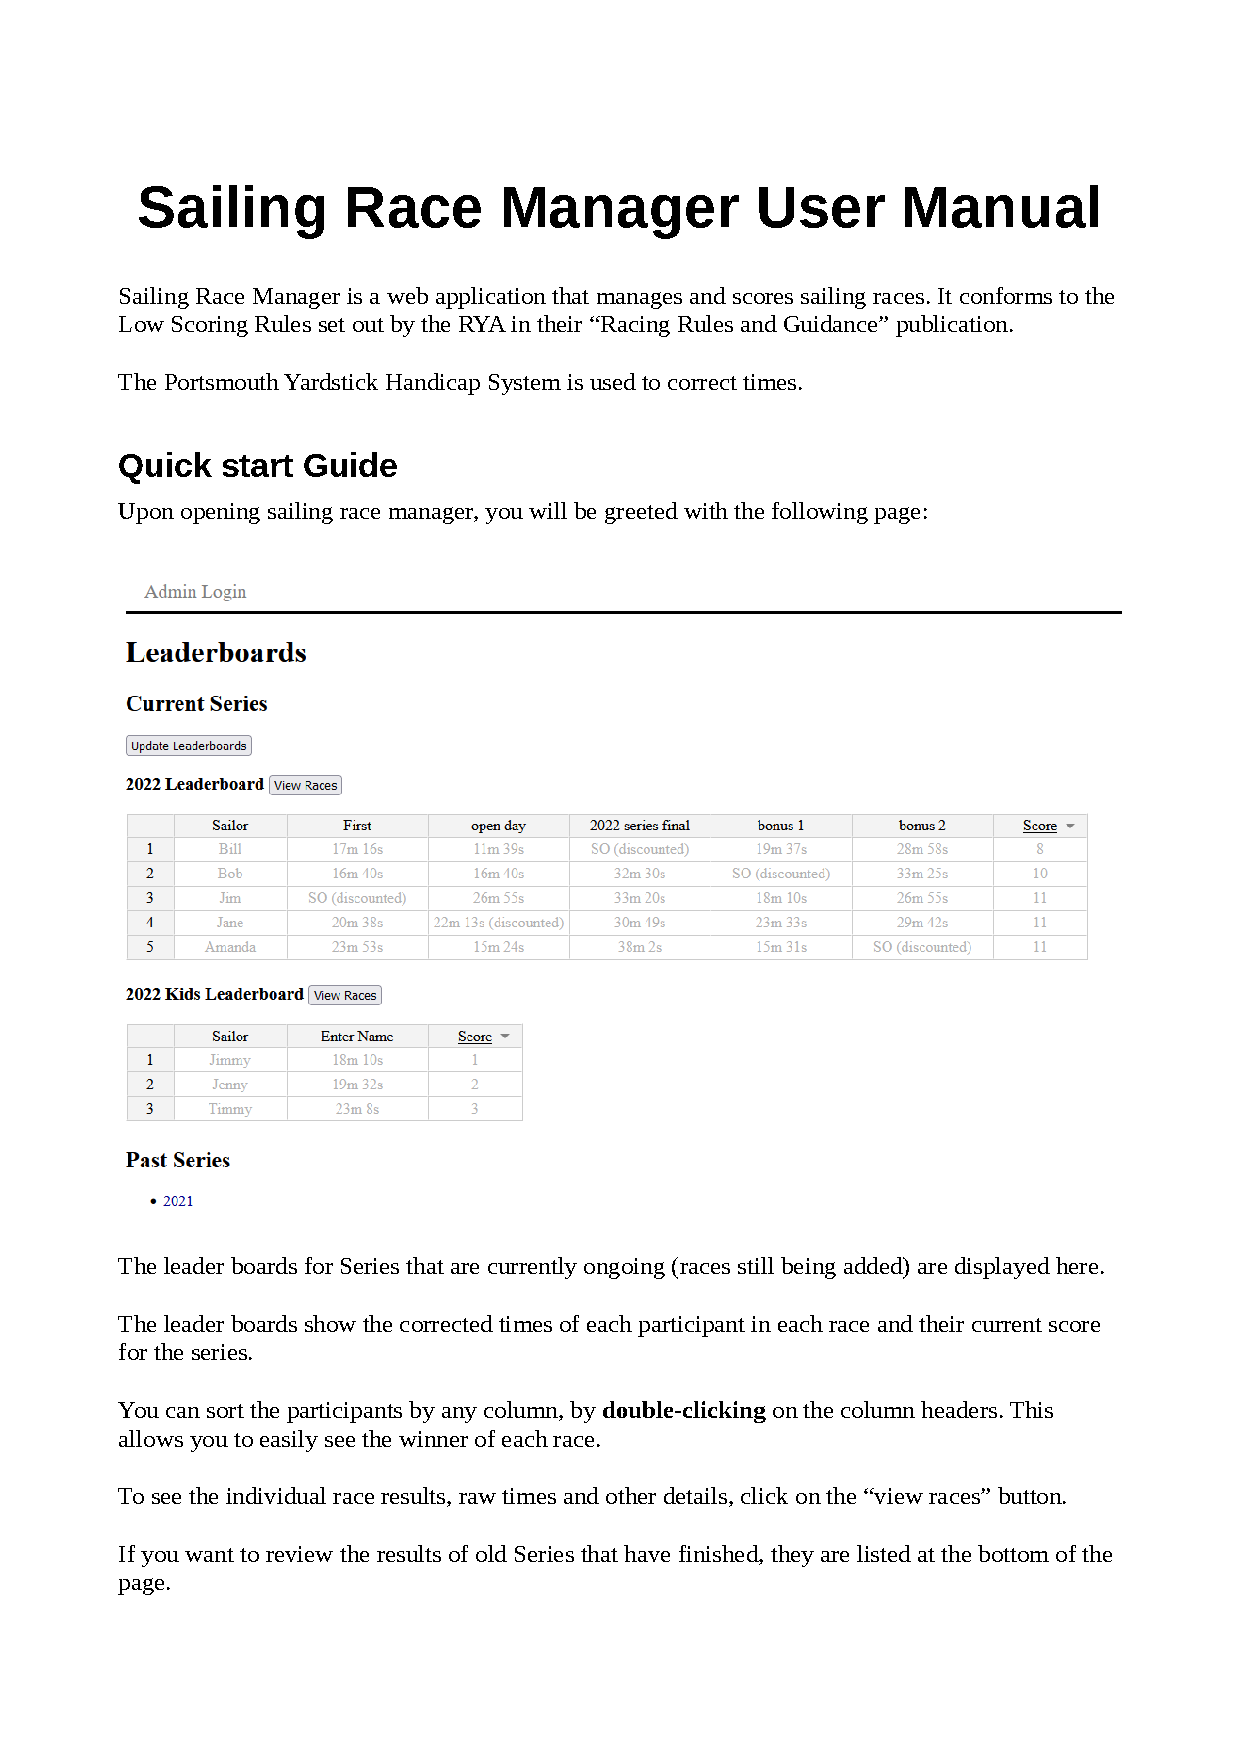
\includepdf[pages=-]{images/User Manual.pdf}

\section{Deployment Manual}
\# Readme

Source code is located under "SailingRaceManger\_project". Within this:

HTML pages are found under "templates"

Django backend files are found under "Sailing Race Manager"

Bundled JavaScript libraries are found under "Sailing Race Manager/static/Sailing Race Manager/Libraries"

\hfill\\
\#\# Build instructions
\hfill\\
\#\#\# Requirements

Python 3

Modern web browser

Packages: listed in `requirements.txt` 

Tested on Windows 10 and Ubuntu Linux

\hfill\\
\#\#\# Build steps

1. Install the required packages with the command:

	pip install -r rquirements.txt

or open the file and install them manually.

2. To create and populate the database with the 2023 Portsmouth Yardstick hanidcap numbers, run the following command from the "SailingRaceManager" folder:

	python populate.py

\hfill\\
\#\#\# Run steps

1. To run the Web App locally, run the following command from the same place:

	python manage.py runserver

2. Navigate to the Url that is given to open the Web App.

\hfill\\
\#\#\# Test steps

1. Follow the steps above in "Run steps", and navigate any web browser to the given URL. If the leader Board page is displayed, the software is working correctly.

2. To run the Automated unit tests, run the following command:

 python manage.py test

\hfill\\
\#\#\# Public hosting

You can easily host the web-App publicly by building a docker image useing the supplied docker file.

The image can be used to host on a provider of your choice.

\hfill\\
\#\# Embedding Leaderboard on another website

To embed the leader board of any series on another website, use an <iframe> html tag and link it to the following URL:

	<Top LevelDomain>/embedded-leaderboard/<Series Name>

To ensure the correct series name is used, navigate to the Sereis editor on your chosen, and get the Series name form the end of the URL. e.g.:


	<Top LevelDomain>/admin-home/series-editor/<Series name is here>



\section{Full Questionnaire} \label{apend:questions}
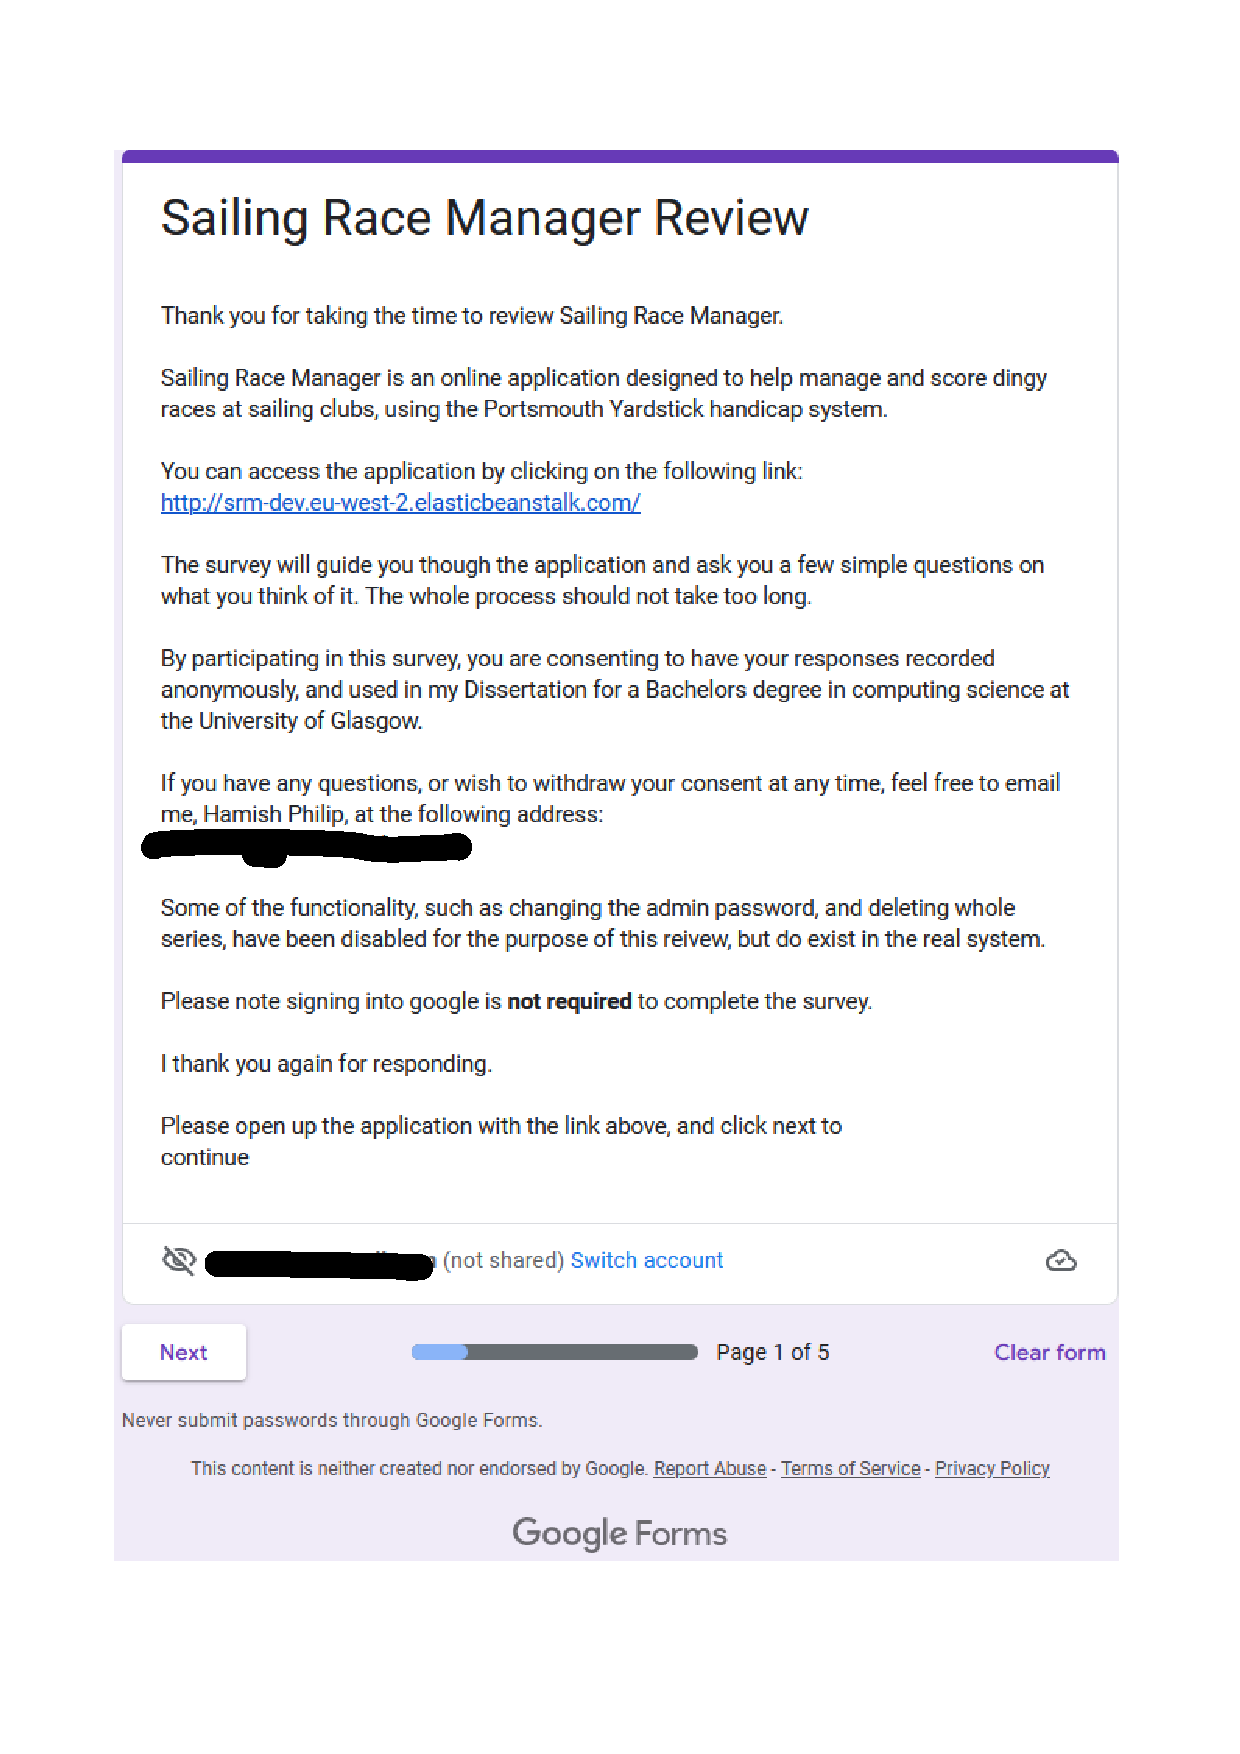
\includepdf[pages=-]{images/Questionaire.pdf}

\section{Raw Results}

\begin{table}[!ht]
    \centering
    \caption{Non-admin Section ratings, from 1-5}
    \begin{tabular}{|l|p{0.8\linewidth}|}
    \hline
        \textbf{Participant} & \textbf{Rateing}  \\ \hline
        1 & 4  \\ \hline
        1 & 5  \\ \hline
        1 & 4  \\ \hline
        1 & 4  \\ \hline
    \end{tabular}
\end{table}

\begin{table}[!ht]
    \centering
    \caption{issues with Non-admin Section responces}
    \begin{tabular}{|l|p{0.8\linewidth}|}
    \hline
        \textbf{Participant} & \textbf{Response}  \\ \hline
        1 &   \\ \hline
        1 & grey type is a bit faint to read  \\ \hline
        1 & Some colour differentiation would be good  \\ \hline
        1 & Some of the table functionality seems to hang  \\ \hline
    \end{tabular}
\end{table}
\begin{table}[!ht]
    \centering
    \caption{Things missing from Non-admin Section responces}
    \begin{tabular}{|l|p{0.8\linewidth}|}
    \hline
        \textbf{Participant} & \textbf{Response}  \\ \hline
        1 & More distinctive colours for table header for easier viewing, however the page is legible regardless  \\ \hline
        1 & no  \\ \hline
        1 & There is no space for sail number or crew to be displayed, which is information some people might like to see  \\ \hline
        1 & Inclusion of more information in the tables would make it more usable -- uncorrected times, corrected times, and points for each erace.  \\ \hline
    \end{tabular}
\end{table}
\begin{table}[!ht]
    \centering
    \caption{Series Editor ratings, from 1-5}
    \begin{tabular}{|l|p{0.8\linewidth}|}
    \hline
        \textbf{Participant} & \textbf{Rating}  \\ \hline
        1 & 4  \\ \hline
        1 & 5  \\ \hline
        1 & 4  \\ \hline
        1 & 4  \\ \hline
    \end{tabular}
\end{table}
\begin{table}[!ht]
    \centering
    \caption{issues with Series Editor responses}
    \begin{tabular}{|l|p{0.8\linewidth}|}
    \hline
        \textbf{Participant} & \textbf{Response}  \\ \hline
        1 &   \\ \hline
        1 & no  \\ \hline
        1 &   \\ \hline
        1 &   \\ \hline
    \end{tabular}
\end{table}
\begin{table}[!ht]
    \centering
    \caption{Things missing from Series Editor responses}
    \begin{tabular}{|l|p{0.8\linewidth}|}
    \hline
        \textbf{Participant} & \textbf{Response}  \\ \hline
        1 &   \\ \hline
        1 &   \\ \hline
        1 & It would be useful to see positions as well as times in the results section. For larger fleets it's not always immediately obvious where someone's time sits in the grand scheme of things.  \\ \hline
        1 &   \\ \hline
    \end{tabular}
\end{table}
\begin{table}[!ht]
    \centering
    \caption{Race Editor ratings, from 1-5}
    \begin{tabular}{|l|p{0.8\linewidth}|}
    \hline
        \textbf{Participant} & \textbf{Rating}  \\ \hline
        1 & 5  \\ \hline
        1 & 4  \\ \hline
        1 & 4  \\ \hline
        1 & 4  \\ \hline
    \end{tabular}
\end{table}
\begin{table}[!ht]
    \centering
    \caption{issues with Race Editor responses}
    \begin{tabular}{|l|p{0.8\linewidth}|}
    \hline
        \textbf{Participant} & \textbf{Response}  \\ \hline
        1 &   \\ \hline
        1 & why is some type black and some grey?  \\ \hline
        1 &   \\ \hline
        1 & Boat dropdown doesn't always work, although dropdown appears if I type into the box  \\ \hline
    \end{tabular}
\end{table}
\begin{table}[!ht]
    \centering
    \caption{Things missing from Series Editor responses}
    \begin{tabular}{|l|p{0.8\linewidth}||}
    \hline
        \textbf{Participant} & \textbf{Response}  \\ \hline
        1 &   \\ \hline
        1 &   \\ \hline
        1 &   \\ \hline
        1 & Nope, all good  \\ \hline
    \end{tabular}
\end{table}





\end{appendices}

%==================================================================================================================================
%   BIBLIOGRAPHY   

% The bibliography style is abbrvnat
% The bibliography always appears last, after the appendices.

\bibliographystyle{abbrvnat}

\bibliography{l4proj}

\end{document}
